% Adaptive DAPP（docs/11 11.11）を基にした論文の骨子
% コンパイル: cd docs/paper/dapp && latexmk -lualatex dapp_outline.tex
% 図の再生成: .venv/bin/python docs/paper/dapp/make_figs.py（施策の単独効果: docs/paper/dapp/measure_effects.py）
\documentclass[a4paper,10pt]{ltjsarticle}
\usepackage[margin=20mm]{geometry}
\usepackage{amsmath,amssymb}
\usepackage{graphicx}
\usepackage{booktabs}
\usepackage{tabularx}
\usepackage{longtable}
\usepackage{enumitem}
\usepackage{xcolor}
\usepackage{float}
\usepackage[section]{placeins}
\usepackage{tikz}
\usetikzlibrary{positioning,arrows.meta,fit}
\usepackage[hidelinks]{hyperref}
\setlist{nosep,leftmargin=1.5em}
\definecolor{cblue}{HTML}{2A78D6}
\definecolor{corange}{HTML}{EB6834}
\definecolor{cgray}{HTML}{52514E}
\newcommand{\todo}[1]{\textcolor{corange}{【#1】}}
\newcolumntype{L}{>{\raggedright\arraybackslash}X}
\renewcommand{\arraystretch}{1.12}

\title{初期行動と状態依存の適応ルールを同時に探索する適応的政策経路（Adaptive DAPP）\\[2pt]
\large ― 計画時の想定（考慮する気候の幅・目標水準）が推奨経路をどう変えるか：阿武隈川流域の流域治水への適用 ―\\[6pt]
\normalsize 論文の骨子（docs/11 第11.11節の実装・計算に基づく草案）}
\author{}
\date{2026年11月9日}

\begin{document}
\maketitle

\begin{abstract}
本資料は、阿武隈川全域（1000 m メッシュ）を対象に実装した Adaptive DAPP（docs/11 第11.11節）に基づき、論文の骨子を整理したものである。
論文の主題は二つある。一つは、深い不確実性の下で、どの初期行動と状態依存の適応ルールの組合せが望ましいか。
もう一つは、その答えが計画時の想定、すなわち計画時に考慮する気候の幅・目標水準・監視情報の質によってどう変わるかである。
あらかじめ与えた経路網の上で施策を切り替える方式（docs/11 第11.9節）は、比較の基準（benchmark）として補足的に扱う。
数値は既存の計算（探索 \texttt{abukuma\_explore\_v2}、Adaptive DAPP \texttt{abukuma\_dapp\_adaptive} と GUI での再計算）による。
遊水地を計画中の阿武隈川上流遊水地群に置き換えた計算（v3・v4）は完了しており、表と図は今後その結果で置き換える（\ref{sec:next}節）。
\end{abstract}

\tableofcontents
\bigskip

%=====================================================================
\section{論文の主張}
\label{sec:claim}

\subsection{背景}
流域治水では、堤防・遊水地などの河川の施策と、田んぼダム・森林化・住宅対策・内水対策などの流域の施策を、
気候変動の進み方に合わせて段階的に組み合わせる必要がある\cite{mlit_ryuiki,mlit_teigen}。
適応的政策経路（DAPP）\cite{haasnoot2013}は、今実施する行動と、どの条件で次の行動に移るかを示す枠組みである。
多くの適用では、経路の候補と切り替えの条件を分析者があらかじめ与える。このため、
(i) 今の行動と将来の切り替え方を一体として選ぶこと、
(ii) 計画時にどの範囲の将来を考え、どの水準の目標を置くかによって望ましい経路がどう変わるかを示すこと、の二つが難しい。

計画時の想定は計画者自身が選ぶものであり、その選び方は計画の結果を左右する。
狭い気候の幅だけを想定すれば計画は安くなるが、想定を超える将来では性能が落ちうる。
目標を高く置けば早い段階での備えが必要になり、将来に施策を追加・修正する余地は小さくなりうる。

関連する研究として、DAPP\cite{haasnoot2013}、Adaptation Tipping Points\cite{kwadijk2010}、RDM\cite{lempert2003}と DAPP の比較\cite{kwakkel2016}、
直接方策探索（EMODPS）\cite{giuliani2016,quinn2017}、監視と signpost の設計\cite{haasnoot2018,hermans2017}がある。
\todo{Real options、国内の流域治水・田んぼダムの効果評価の文献を追加}

\subsection{リサーチクエスチョン}
\begin{enumerate}
  \item[RQ1] Which combinations of initial actions and state-dependent adaptation rules are preferred under deep uncertainty?\\
    深い不確実性の下で、どの初期行動と状態依存の適応ルールの組合せが望ましいか。
  \item[RQ2] How does the preferred adaptive pathway change with the breadth of future conditions considered during planning?\\
    計画時に考慮する将来の幅によって、望ましい適応経路はどう変わるか。
  \item[RQ3] How do pathways designed under different planning assumptions perform under a common broader evaluation ensemble?\\
    異なる計画時の想定で設計した経路は、共通のより広い評価シナリオの下でどう機能するか。
  \item[RQ4] How does target ambition change the balance between early preparedness and future flexibility?\\
    目標の水準は、早い段階の備えと将来の柔軟性の釣り合いをどう変えるか。
\end{enumerate}
感度の主な軸は、計画時に考慮する気候の幅（planning climate range）・目標の水準（Target）・監視情報の質（information quality）の三つである（\ref{sec:axes}節）。

\subsection{主張（現時点の結果からの仮説）}
\begin{itemize}
  \item \textbf{RQ1}: 初期行動ごとに最良の適応ルールを探索すると、Coverage と費用のトレードオフの上に、
    初期費用の小さい初期行動（施策なし・\#1・\#2; 0〜250 億円）と、初期費用の大きい初期行動（\#73・\#5; 約 425 億円）が並ぶ。
    望ましいルールの多くは、被害の観測値・予測値と降雨の傾向を監視し、Target の 0.7〜0.9 倍に達した時点で次の行動を始める。
  \item \textbf{RQ2}: 考慮する気候の幅を変えても推奨される初期行動は変わらず（\#2, 250 億円）、変わるのはその後のルールである。
    穏やかな気候（Low）だけを考えると被害の観測値だけを監視して遅めに動き、厳しい気候（High）だけを考えると予測値も監視して早めに動く。
    厳しい気候を考えるほど平均費用は増える（345 → 523 億円）。
  \item \textbf{RQ3}: 共通の評価シナリオで評価すると、狭い範囲で設計した経路ほど、計画時に見込んだ性能と実際の性能の差が大きい
    （Low: 見込み 100\% に対し 53\%）。全範囲（Low–High）で設計した経路は差が小さい（見込み 71\%、評価 66\%）。
  \item \textbf{RQ4}: 目標の水準は、気候の幅よりも推奨経路を大きく変える。被害額の Target を 1.4 倍に緩めると初期費用の大きい \#73（423 億円）が推奨され、
    残る将来の選択肢は少なくなる（47〜54\%）。1.0 倍に厳しくすると、どの初期行動でも Target を保てる将来が少なくなり（Coverage 34〜48\%）、
    初期費用の小さい初期行動（\#1・\#2）が選ばれて、選択肢は多く残る（56〜73\%）。
  \item 監視情報の質（観測誤差・予測誤差・傾向の推定に使う観測数）の影響は小さい（Coverage の変化は 1〜2 pt）。
\end{itemize}

\subsection{新規性}
\begin{enumerate}
  \item 初期行動と状態依存の適応ルール（監視指標・トリガー・次の行動の選び方・縮小）を同時に探索し、ルールが生む分岐全体を一つの DAPP として評価する。経路の候補はあらかじめ与えない。
  \item 計画時の想定（考慮する気候の幅・目標の水準・監視情報の質）を設計の条件として変え、設計した経路を共通の広い評価シナリオで評価する。これにより、計画時に見込んだ性能と実際の性能の差を示す。
  \item 分布型降雨流出氾濫モデル（RRI）と資産に基づく被害推計を代理モデルでつなぎ、施策の実施過程（合意・施工・普及・成熟、予算の繰越、変更費用、土地利用の不可逆性）を持つ実施モデルの上で経路を模擬する。
\end{enumerate}

%=====================================================================
\section{対象流域とモデル}
\label{sec:model}

\begin{itemize}
  \item 対象: 阿武隈川全域（流域面積 約5,400 km\textsuperscript{2}）、1000 m メッシュ。地域区分は観測所の集水域の入れ子
    （上流＝本宮より上流、中流＝伏黒まで、下流＝それより下流）。
  \item 物理モデル: RRI 型の分布型降雨流出氾濫モデル\cite{sayama2012}（docs/01）。代表洪水は令和元年東日本台風。
    被害額はメッシュごとの資産（建物・家財・農作物等）と浸水深から治水経済調査マニュアル\cite{mlit_manual}に従って推計する（docs/03）。
    対策なし・現在気候の被害額 756 億円。式とパラメータは\ref{sec:formulation}節に示す。
  \item 代理モデル: 探索（docs/12）で RRI を 547 回実行し、施策の水準・効果係数・気候（降雨倍率・海面上昇・降雨強度の強調 γ）を入力、
    被害額・浸水人口・Ecology・Livability を出力とするガウス過程（GP）を学習した。検証は被害額 $R^2$ 0.99、相対 RMSE 3.3\%、目標判定の一致率 99\%。
  \item 実施モデル（docs/13 \texttt{roadmap.sim.State}）: 2020〜2100 年を 10 年ごとの意思決定、5 年ごとの評価で模擬する。
    施策は合意形成 → 施工／植栽 → 普及 → 成熟の段階を経て効果を持ち、初期費用・維持費・変更費用を持つ。予算（初期費用の総額 2,000 億円・10 年ごと 500 億円, 仮定）を超える分は次の期へ繰り越す。
    社会過程（合意の失敗・参加率）はこの分析では扱わない（全員参加・失敗なし）。
\end{itemize}

%=====================================================================
\section{被害額と施策効果の定式化}
\label{sec:formulation}

本節は実装（\texttt{rri\_sim}: \texttt{solver.py}・\texttt{damage.py}・\texttt{gui/engine.py}・\texttt{rdm/candidates.py}・\texttt{rdm/evaluate.py}・\texttt{costs.py}・\texttt{roadmap/sim.py}）の式とパラメータをまとめる。
施策の表現は遊水地を除いて探索 v2〜v4 で共通であり、遊水地は v3 以降の計画中の遊水地群による（\ref{sec:meas-model}節）。
「仮定」と記した値は根拠となる観測・事業資料がなく、効果係数・費用の不確実性として扱う。

\subsection{降雨流出氾濫モデル}
斜面（2 次元, 1000 m 格子, D4）では、RRI モデル\cite{sayama2012}と同じく表層土壌中の水と地表水をまとめた貯留水深 $h$ の連続式と流量–水深関係を解く:
\begin{equation}
\frac{\partial h}{\partial t}+\frac{\partial q_x}{\partial x}+\frac{\partial q_y}{\partial y}=r-f,\qquad
q=\begin{cases}
k_m d_m (h/d_m)^{\beta}\, i & (h\le d_m)\\
\{k_m d_m + k_a(h-d_m)\}\, i & (d_m<h\le d_a)\\
\{k_m d_m + k_a(d_a-d_m)\}\, i + \dfrac{1}{n}(h-d_a)^{5/3} i^{1/2} & (d_a<h)
\end{cases}
\label{eq:slope}
\end{equation}
ここで $i$ は水面勾配、$d_a=D\gamma_a$・$d_m=D\gamma_m$（$D$: 土層厚、$\gamma_a$・$\gamma_m$: 有効・不飽和間隙率）、$k_m=k_a/\beta$、$n$ は等価粗度である。
鉛直浸透 $f$ は Green–Ampt 式\cite{greenampt1911} $f=k_v\{1+(\phi-\theta_i)S_f/F\}$（累積浸透量 $F$ に上限 $F_{\max}$）による。
河道（1 次元）は矩形断面の連続式と Manning 式 $Q=n_r^{-1}AR^{2/3}|\partial H/\partial x|^{1/2}$ で、
川幅・深さを上流域面積 $A_{up}$ [km\textsuperscript{2}] から $W=5.0A_{up}^{0.35}$, $D_r=0.95A_{up}^{0.2}$ と与える。
河道と斜面の水交換は、天端高 $z_c=z+E$（$E$: 堤防高）を越える側から本間の越流公式\cite{honma1940}
（完全越流 $q=0.35h_1\sqrt{2gh_1}$、もぐり越流 $q=0.91h_2\sqrt{2g(h_1-h_2)}$、越流長は河道長 × 2）で与える。
運動量は局所慣性近似\cite{bates2010}で摩擦項を陰的に扱い、水収支は丸め誤差の範囲で保存する。
浸水と被害の対象は HAND\cite{renno2008,nobre2011}（最寄り河道からの比高）$\le 10$ m かつ最大浸水深 $\ge 0.1$ m のセルに限る。

土地利用クラスのパラメータを表\ref{tab:landparams}に示す（阿武隈川では流域の較正を行わず事前値を用いた。須賀川の 2019 年の流量で NSE 0.98, docs/04）。

\begin{table}[tbp]
\centering\footnotesize\setlength{\tabcolsep}{3pt}
\caption{Parameters of the land-use classes (\texttt{basin.default\_land\_params}, \texttt{workflow.model\_land\_params}). Lower block: classes created by measures}
\label{tab:landparams}
\begin{tabular}{@{}lrrrrrrrr>{\raggedright\arraybackslash}p{30mm}@{}}
\toprule
Class & $n$ & $k_a$ [m/s] & $D$ [m] & $\gamma_a$ & $\gamma_m$ & $k_v$ [m/s] & $\phi-\theta_i$ & $S_f$ [m] & Other \\
\midrule
Forest & 0.40 & 0.1 & 1.0 & 0.4 & 0.1 & -- & -- & -- & $\beta=8$ \\
Paddy field & 0.30 & -- & -- & -- & -- & $2\times10^{-7}$ & 0.2 & 0.1 & $F_{\max}=0.05$ m \\
Upland field & 0.20 & -- & -- & -- & -- & $5\times10^{-6}$ & 0.3 & 0.2 & $F_{\max}=0.3$ m \\
Built-up & 0.05 & -- & -- & -- & -- & $1\times10^{-7}$ & 0.1 & 0.1 & $F_{\max}=0.01$ m \\
Water & 0.03 & -- & -- & -- & -- & -- & -- & -- & \\
\midrule
Paddy-field dam & 0.30 & -- & -- & -- & -- & \multicolumn{3}{c}{as paddy field} & retains $s_P=0.15k_P$ m, releases 5 mm/h when full \\
New forest (afforestation) & $0.25+0.15k_F$ & 0.05 & $1.0k_F$ & 0.4 & 0.1 & -- & -- & -- & $\beta=8$ \\
Green space (relocated sites) & 0.30 & -- & -- & -- & -- & \multicolumn{3}{c}{as upland field} & \\
Wetland (retention basin) & 0.10 & -- & -- & -- & -- & \multicolumn{3}{c}{as paddy field} & excluded from inundation and damage \\
\bottomrule
\end{tabular}
\end{table}

\paragraph{気候の与え方}
将来の降雨は、代表洪水の観測降雨 $r_i(t)$（セル $i$）を総雨量の倍率 $\alpha$ と強雨の強調 $\gamma$ で変換する:
\begin{equation}
r'_i(t)=c_i\,r_i(t)^{\gamma},\qquad \textstyle\sum_t r'_i(t)\,\Delta t=\alpha\sum_t r_i(t)\,\Delta t .
\label{eq:rain}
\end{equation}
$\gamma=1$ は一様な倍率で、$\gamma>1$ は総雨量を変えずに強い雨に増分を集中させる。海面上昇 $\Delta\eta$ は河口の潮位境界に加える。
$\alpha$ の幅は治水計画の降雨量変化倍率（2℃ 上昇で 1.1）\cite{mlit_teigen}、$\Delta\eta$ は日本の気候変動 2020\cite{jma2020}（東北・21 世紀末 2℃ 0.38 m・4℃ 0.70 m）による（表\ref{tab:unc}）。

\subsection{被害額と浸水人口}
\label{sec:damage}
直接被害額は治水経済調査マニュアル（案）（令和 7 年 6 月改正, 令和 5 年評価額）\cite{mlit_manual}に従い、資産額と浸水深別の被害率の積の和とする:
\begin{equation}
D=\sum_{i}\Bigl[\sum_{c\in\mathcal{G}} V_{i,c}\,\rho_c\bigl(h_i-h^{f}_i;\,s_i\bigr)+V_{i,\mathrm{car}}\,\rho_{\mathrm{car}}(h_i)
+\sum_{c\in\{\text{水稲},\text{畑}\}} V_{i,c}\,\rho_c(h_i,\tau_i)\Bigr].
\label{eq:damage}
\end{equation}
$\mathcal{G}$ は家屋・家庭用品・事業所の償却資産と在庫・農漁家の償却資産と在庫、$h_i$ は最大浸水深、$h^f_i$ は床高（既定 0.45 m; 嵩上げで増える）、
$s_i$ は地盤勾配の群（A: $<1/1000$, B: $1/1000$〜$1/500$, C: $\ge1/500$; DEM 勾配を 3×3 で平滑化）、$\tau_i$ は浸水日数（浸水深 $\ge0.1$ m の時間 ÷ 24）である。
床上の被害率は床面からの浸水深を 0.5・1・2・3 m で区切った 5 区分、床下（$0<h<h^f$）は 1 区分とする（表\ref{tab:damrate}）。

1 km 格子のセル内では地盤高が大きく異なるため、セル内の 100 m 土地利用メッシュの地盤高（5 m 標高）の 20 分位 $z_{i,q}$ を
建物用地・農地ごとに保持し、セルの水量 $h_i A$ を全メッシュの標高分布に入れたときの水位 $H_i$ から、
分位ごとの浸水深 $h_{i,q}=\max(H_i-z_{i,q},0)$ で式(\ref{eq:damage})を評価して平均する（docs/03 §3.2-9）。

資産額 $V$ は、家屋＝延床面積 × 247.1 千円/m\textsuperscript{2}（福島県, 第 1 表）、家庭用品＝世帯数 × 9,368 千円、自動車＝世帯数 × 3,502 千円、
事業所＝産業大分類別の従業者数 × 第 3 表の単価、農漁家＝農家数 × 3,110（償却）・981（在庫）千円/戸、
水稲＝水田面積 × 532 kg/10a × 187 千円/t、畑作物＝畑面積 × 22.3 千円/a（令和 2 年の耕種−米の産出額 ÷ 畑面積）である。
世帯数・従業者数・農家数は国勢調査（250 m）・経済センサス（500 m）・農林業センサス（1 km）、土地利用は国土数値情報 L03-b\cite{ksj}による。

浸水人口は最大浸水深 0.5 m 以上のセルの人口 $P=\sum_i \mathrm{pop}_i\,\mathbf{1}(h_i\ge0.5\ \mathrm{m})$ とする。
2020〜2100 年の各評価年 $t$ では、代理モデルの予測に資産係数 $a(t)$・人口係数 $p(t)$（表\ref{tab:unc}; 変化開始年から 2100 年まで線形）を掛ける:
$D_t=a(t)\,\hat D(\boldsymbol\phi_t)$、$P_t=p(t)\,\hat P(\boldsymbol\phi_t)$（\ref{sec:surrogate}節）。

\begin{table}[tbp]
\centering\footnotesize\setlength{\tabcolsep}{4pt}
\caption{Damage ratios (Manual for Economic Evaluation of Flood Control\cite{mlit_manual}, Tables 4.2--4.6)}
\label{tab:damrate}
\begin{tabular}{@{}lrrrrrr@{}}
\toprule
Asset (depth above floor) & Below floor & $<0.5$ m & 0.5--1 & 1--2 & 2--3 & $\ge3$ m \\
\midrule
House, group A (slope $<1/1000$) & 0.047 & 0.189 & 0.253 & 0.406 & 0.592 & 0.800 \\
House, group B ($1/1000$--$1/500$) & 0.058 & 0.219 & 0.301 & 0.468 & 0.657 & 0.843 \\
House, group C ($\ge1/500$) & 0.064 & 0.235 & 0.325 & 0.499 & 0.690 & 0.865 \\
Household goods & 0.037 & 0.308 & 0.533 & 0.701 & 0.948 & 0.977 \\
Business, depreciable & 0.064 & 0.296 & 0.573 & 0.801 & 0.920 & 0.940 \\
Business, inventory & 0.053 & 0.282 & 0.440 & 0.814 & 0.946 & 0.975 \\
Farm/fishery household, depreciable & 0 & 0.113 & 0.327 & 0.483 & 0.828 & 1.000 \\
Farm/fishery household, inventory & 0 & 0.223 & 0.584 & 0.618 & 0.792 & 0.942 \\
\bottomrule
\end{tabular}
\par\footnotesize\raggedright Cars (depth above ground): $<0.3$ m 0, 0.3--0.5 m 0.1, 0.5--0.7 m 0.5, $\ge0.7$ m 1.0.
Crops (depth × duration of 1--2/3--4/5--6/$\ge$7 days): rice $<0.5$ m 0.21/0.30/0.36/0.50, 0.5--1 m 0.24/0.44/0.50/0.71, $\ge1$ m 0.37/0.54/0.64/0.74;
upland crops (average) $<0.5$ m 0.27/0.42/0.54/0.67, 0.5--1 m 0.35/0.48/0.67/0.74, $\ge1$ m 0.51/0.67/0.81/0.91.
Sediment deposition ratios and the storey correction are not applied (no sediment model; no data on the mean number of storeys).
\end{table}

\subsection{施策の効果の表現}
\label{sec:meas-model}
各施策は RRI の入力（地形・河道・土地利用クラス・資産・境界条件）の変更として表し、効果は代表洪水の再計算で得る（表\ref{tab:measmodel}）。
施策の対象セルは対策なし・現在気候の計算（基準計算）の結果と地形から決め、効果係数 $k$（表\ref{tab:unc}）は施策の物理量に掛ける。
施策の分類と内容は流域治水の施策体系\cite{mlit_ryuiki}に対応させた。

\begin{table}[tbp]
\centering\footnotesize\setlength{\tabcolsep}{3pt}
\caption{Representation of the measures in the model (1000 m grid; numbers of cells: upstream/midstream/downstream; v4)}
\label{tab:measmodel}
\begin{tabularx}{\textwidth}{@{}>{\raggedright\arraybackslash}p{20mm} >{\raggedright\arraybackslash}p{38mm} L >{\raggedright\arraybackslash}p{30mm}@{}}
\toprule
Measure & Target cells & Representation (parameters) & Effect coefficient $k$ scales \\
\midrule
Levee raising & River cells with catchment $\ge5$ km\textsuperscript{2} and baseline peak water level $\ge$ crest $-0.2$ m (48/3/40) &
  Levee height $E\leftarrow E+k_L\Delta H$ ($\Delta H\in\{1,2\}$ m); raises the crest of the overflow (Honma) & Raised height (gaps, settlement, weak sections)\\
Retention basin (Upper Abukuma retention basins) & Farmland/forest next to a river with catchment $\ge300$ km\textsuperscript{2} within 2.5 km of the planned sites (Kagamiishi, Tamakawa, Yabuki), 4 cells in order of HAND &
  Off-channel storage with an overflow weir. Capacity $V=k_R V_0$, $V_0=15\times10^6$ m\textsuperscript{3}, site 350 ha\cite{mlit_usuichi} (mean depth 4.3 m); Eq.~(\ref{eq:retention}) & Capacity (operation, sedimentation)\\
Paddy-field dam & Share $x$ of all paddy cells of the zone (408/70/190; random order) &
  Outlet boards retain surface water up to $s_P=0.15k_P$ m (not moved by overland flow), released as a linear reservoir $\mathrm{d}S/\mathrm{d}t=-\lambda S$ ($\lambda=5\,\mathrm{mm/h}/s_P$; 5 mm/h when full)\cite{maff_tanbo} & Storage depth (participation, outlet management)\\
Afforestation & Share $x$ of paddy/upland fields with HAND $\ge20$ m (60/49/26) &
  Converted to the new-forest class (Table~\ref{tab:landparams}: $n=0.25+0.15k_F$, $D=1.0k_F$ m); crop assets removed & Increase in roughness and soil depth (maturity)\\
House raising & Cells with households and baseline depth $\ge1$ m (1/--/4) &
  Floor height $h^f\leftarrow 0.45+k_H\cdot1.0$ m (changes the above/below-floor classes in Eq.~(\ref{eq:damage})) & Raised height (implementation rate)\\
Relocation & As above &
  Households, employees and assets moved to new sites on high ground (HAND $>10$ m, dry in the baseline, gentle slope; 40 persons/ha); vacated land becomes green space & --- \\
Urban drainage pump & Built-up cells with HAND $\le5$ m and baseline depth $\ge0.1$ m (5/--/15) &
  Surface water pumped to the receiving river cell at $\le\rho_d=10$ mm/h regardless of river stage: $\Delta h_i=\min(h_i-d_a-s_i,\ \rho_d\Delta t)$ & --- \\
Agricultural drainage pump & Farmland cells, same criteria (40/--/70) & As above, $\rho_d=3$ mm/h & --- \\
Public rainwater storage & Built-up cells with baseline depth $\ge0.1$ m (5/--/15) & Additional retained depth 30 mm, released at 2 mm/h when full (linear reservoir) & --- \\
Household rainwater storage & Share $x$ of the above & Retained depth 10 mm, 2 mm/h when full & --- \\
\bottomrule
\end{tabularx}
\par\footnotesize Zones are nested gauge catchments (upstream: above Motomiya; midstream: down to Fushiguro; downstream: below).
\end{table}

\paragraph{遊水地}
遊水地は流入地点（用地から 1 km 以内で最大の河道セル）の流量 $Q_{\mathrm{in}}(t)$ のうち越流開始流量 $Q_c$ を超える分を取り込む河道外の貯留とする:
\begin{equation}
Q_{\mathrm{out}}=\min(Q_{\mathrm{in}},Q_c),\quad
\frac{\mathrm{d}S}{\mathrm{d}t}=
\begin{cases}
\max(Q_{\mathrm{in}}-Q_c,0) & (S<V)\\
-\min\bigl(S/\Delta t,\ 0.5Q_c-Q_{\mathrm{in}}\bigr) & (Q_{\mathrm{in}}<0.5Q_c)
\end{cases}
\label{eq:retention}
\end{equation}
（満水後は素通り）。$Q_c$ は基準計算（現在気候）の流入地点の流量 $Q^0(t)$ について $\int\max(Q^0-Q_c,0)\,\mathrm{d}t=V$ となる値
（この洪水で容量がちょうど満杯になる値; 完全予見の運用）とする。用地は湿地クラスとし、被害・浸水の集計から除き、用地内の世帯は移転させる。
探索 v2 以前は、自動選定した下流の 3 か所（各 1 セル、貯留深 3 m × 効果係数）を別々の変数としていた。

\paragraph{効果係数と技術変化}
探索（代理モデルの学習）では効果係数を $k\in[k_{\mathrm{low}},1]$ の一様乱数とし、実施モデルの将来シナリオでは名目値
（堤防 0.9・遊水地 0.85・田んぼダム 0.6・森林化 0.6・嵩上げ 0.8）を中心とする範囲（表\ref{tab:unc}）から引き、技術変化 $\Delta_k$ を
$k(t)=k_0+\Delta_k\,\mathrm{clip}\bigl((t-t_{\mathrm{tech}})/10,0,1\bigr)$ として加える。田んぼダムの係数の幅は取組率・排水口管理のばらつきを、
森林化は植栽後の成熟度と、大規模洪水では森林の洪水緩和機能が限られるという評価\cite{scj2001,kuraji2004}を想定した仮定である。

\subsection{実施過程と代理モデルへの入力}
\label{sec:surrogate}
施策 $i$ が意思決定年 $t_d$ に水準 $x^{\mathrm{old}}\to x^{\mathrm{new}}$ へ変更されると、合意期間 $C$ の後に次の形で効果を持つ（\texttt{roadmap/sim.py}）:
\begin{align}
\text{(a) 施工型}:&\quad x_i(t)=x^{\mathrm{old}}+(x^{\mathrm{new}}-x^{\mathrm{old}})\,\mathbf{1}(t\ge t_d+C+T_b),\\
\text{(b) 普及型}:&\quad x_i(t)=x^{\mathrm{old}}+(x^{\mathrm{new}}-x^{\mathrm{old}})\,\mathrm{clip}\Bigl(\frac{t-t_d-C}{T_u},0,1\Bigr),\\
\text{(c) 森林化}:&\quad \ell_i(t)=x^{\mathrm{new}}\,\mathrm{clip}\Bigl(\frac{t-t_d-C}{T_b},0,1\Bigr),\\
&\quad e_i(t)=\ell_i(t)\,\mathrm{clip}\Bigl(\frac{t-t_d-C-T_b/2}{T_m},0,1\Bigr).
\end{align}
(a) は堤防・遊水地・排水施設・公共貯留、(b) は田んぼダム・住宅対策・各戸貯留（$x^{\mathrm{new}}$ には取組率の上限を含む）である。
$T_b$・$T_u$・$T_m$ は施工・普及・成熟の期間（表\ref{tab:unc}）、$\ell$ は植栽済みの面積率、$e$ は効果を持つ面積率である。
代理モデルの入力 $\boldsymbol\phi$ は、効果係数を施策の量に掛けた物理的な尺度（施策がなければ係数は効かない）と気候の 3 変数である:
\begin{equation}
\begin{aligned}
\boldsymbol\phi=\Bigl(&\tfrac{\Delta H}{2}k_L,\ \mathbf{1}_{\text{遊水地}}k_R,\ x_{\text{田}}k_P,\ (e_{\text{森}}k_F,\ \ell_{\text{森}}),\\
&(x_{\text{嵩上げ}}k_H,\ x_{\text{移転}}),\ x_{\text{排水・貯留}},\ \tilde\alpha,\ \Delta\tilde\eta,\ \tilde\gamma\Bigr)
\end{aligned}
\end{equation}
（$\tilde\cdot$ は探索範囲で $[0,1]$ に正規化）。出力ごとに $\log(1+D)$ 等を ARD 二乗指数カーネルのガウス過程\cite{rasmussen2006}で回帰し、
リッジ回帰と一つ抜き交差検証の誤差で比べて良い方を使う。学習点は施策・不確実性の LHS\cite{mckay1979}（v2: 320 点）、対策なし（16 点）、
目標の境界付近の適応追加と検証点で、RRI は v2 で 547 回、v4 で 627 回（施策を 1〜3 個だけ入れた 80 点を追加）である。

\subsection{費用}
\label{sec:cost}
費用は施策の物理量 × 単価（表\ref{tab:unitcost}）で、現在価値は $C_{\mathrm{PV}}=C_0+C_a\sum_{y=1}^{50}1.04^{-y}$（年費用 $C_a$, 50 年・4\%）とする（表\ref{tab:measures}）。
実施モデルでは、初期費用を施工・普及の期間に配分し、維持費は毎年計上して 4\% で割り引く。
堤防の嵩上げは、天端幅 $b=5$ m・法勾配 $m=2$ の台形断面 $S(h)=h(b+mh)$ と敷幅 $W(h)=b+2mh$ から、
$C_0=L\{[S(h_0+\Delta H)-S(h_0)]c_{\mathrm{fill}}+c_{\mathrm{fix}}+[W(h_0+\Delta H)-W(h_0)]c_{\mathrm{land}}\}$（$L$: 両岸の延長、$h_0$: 既存の堤防高）とする。
遊水地は $C_0=V c_{\mathrm{exc}}+A c_{\mathrm{land}}+\sqrt{A}\,c_{\mathrm{weir}}+N_{\mathrm{hh}}c_{\mathrm{reloc}}$（$A$: 用地面積、越流堤長 $\sqrt{A}$）で、
上流遊水地群は 496.5 億円となる。排水ポンプ・排水機場の能力は対象セルの面積 × 排水強度の和（m\textsuperscript{3}/s）である。

\begin{table}[tbp]
\centering\footnotesize
\caption{Unit costs (\texttt{costs.py}; assumed unless stated)}
\label{tab:unitcost}
\begin{tabularx}{\textwidth}{@{}l r L@{}}
\toprule
Item & Unit cost & Basis \\
\midrule
Levee fill $c_{\mathrm{fill}}$ / ancillary works $c_{\mathrm{fix}}$ & 8,000 JPY/m\textsuperscript{3} / 50,000 JPY/m & Excavation unit cost (319--777 JPY/m\textsuperscript{3}, design documents) plus material, haulage and compaction \\
Land $c_{\mathrm{land}}$ & 5,000 JPY/m\textsuperscript{2} & Typical price of rural farmland and forest \\
Retention excavation and embankment $c_{\mathrm{exc}}$ / weir $c_{\mathrm{weir}}$ & 1,500 JPY/m\textsuperscript{3} / 1 M JPY/m & As above plus haulage and disposal \\
Paddy-field dam boards / maintenance & 5,000 JPY/10a / 400 JPY/10a/yr & A few thousand JPY per board; paddy-field-dam subsidy of the multifunctional payment \\
Afforestation planting / lost farm income & 1.5 M JPY/ha / 0.266 M JPY/ha/yr & Lost income = 4.75 t/ha × 187 kJPY/t × income ratio 0.3 \\
Relocation & 20 M JPY/household, 3 M JPY/employee & Group relocation projects, price-adjusted \\
House raising (floor) & 6 M JPY/household/m & House lifting \\
Drainage pump & 300 M JPY/(m\textsuperscript{3}/s), maintenance 2\%/yr & Typical cost of drainage pump stations \\
Rainwater storage public / household & 50 k / 100 k JPY/m\textsuperscript{3}, maintenance 500 JPY/m\textsuperscript{3}/yr & \\
\bottomrule
\end{tabularx}
\end{table}

%=====================================================================
\section{施策のリストと効果}
\label{sec:measures}

意思決定変数は 22（9 種類 × 地域）、行動の候補（追加・強化・変更・縮小）は 43 である。
表\ref{tab:measures} に、各施策の最大水準の初期費用・年費用と、\textbf{単独の効果}（他の施策なし、名目の効果係数、代表洪水; 代理モデル）を示す。
基準（対策なし）の被害額は 現在気候 747 億円・4℃相当（降雨 ×1.2・海面 +0.54 m）1,338 億円、浸水人口は 3,394 人・17,819 人（代理モデル）。

\begin{table}[tbp]
\centering\scriptsize\setlength{\tabcolsep}{2.5pt}
\caption{Measures and their single effects (surrogate of \texttt{abukuma\_explore\_v2}; costs from \texttt{costs.py}, 100 M JPY; PV over 50 years at 4\%)}
\label{tab:measures}
\begin{tabularx}{\textwidth}{@{}>{\raggedright\arraybackslash}p{24mm} >{\raggedright\arraybackslash}p{19mm} >{\raggedleft\arraybackslash}p{13mm} >{\raggedleft\arraybackslash}p{10mm} >{\raggedleft\arraybackslash}p{13mm} >{\raggedleft\arraybackslash}p{14mm} >{\raggedleft\arraybackslash}p{14mm} L@{}}
\toprule
Measure, zone & Level & Initial & Annual & \multicolumn{2}{c}{Change in damage} & Flooded pop. & Duration (nominal, range) / reversibility \\
 & & cost & cost & Current & 4\,\textdegree C & Current & \\
\midrule
Levee, upstream & +1/+2 m & 170/292 & 0 & $-11$/$-21$ & $-23$/$-46$ & $-1{,}003$ & Consensus 2 + construction 8 (6--12) yr / never lowered \\
Levee, midstream & +1/+2 m & 10/18 & 0 & ±0\textsuperscript{*} & ±0\textsuperscript{*} & $-30$ & Same \\
Levee, downstream & +1/+2 m & 136/233 & 0 & $-31$/$-28$ & $-80$/$-123$ & $-104$ & Same \\
Retention basins 1--3, downstream & Depth 3 m & 110--180 & 0 & ±0\textsuperscript{*} & $-6$--±0 & ±0 & Consensus 3 + construction 7 (2--12) yr / irreversible (farmland → basin) \\
Paddy-field dam, upstream & 0--100\% & 12 & 0.9 & $-101$ & $-96$ & $-847$ & Consensus 1 + diffusion 9 (4--19) yr / can be scaled back \\
Paddy-field dam, midstream & 0--100\% & 2 & 0.1 & ±0\textsuperscript{*} & ±0\textsuperscript{*} & ±0 & Same \\
Paddy-field dam, downstream & 0--100\% & 6 & 0.4 & $-85$ & $-78$ & $-16$ & Same \\
Afforestation, upstream & 0--100\% & 90 & 10.4 & $-31$ & $-26$ & $-222$ & Consensus 2 + planting 5 + maturity 30 (20--40) yr / back to farmland within 10 yr at 50\% of planting cost \\
Afforestation, mid/downstream & 0--100\% & 74/39 & 8.3/4.1 & ±0\textsuperscript{*}/$-4$ & $-6$/$-12$ & $-30$/$-94$ & Same \\
Housing, upstream & Raising +1 m/relocation & 2/23 & 0 & $-21$/$-29$ & $-16$/$-55$ & ±0 & Consensus 2 + 6 (3--18) yr / consensus 3 + 9 (2--17) yr; raising → relocation allowed, relocation irreversible \\
Housing, downstream & Raising +1 m/relocation & 22/86 & 0 & $-6$/$-27$ & $-12$/$-56$ & $-1{,}223$ & Same \\
Urban drainage pump & +10 mm/h (up/down) & 42/125 & 0.8/2.5 & $-19$/$-56$ & $-19$/$-49$ & $-56$/$-155$ & Construction 4--12 yr \\
Agricultural drainage pump & +3 mm/h (up/down) & 100/175 & 2.0/3.5 & $-5$/$-33$ & $-10$/$-20$ & $-366$/$-40$ & Construction 4--12 yr \\
Public rainwater storage & 30 mm (up/down) & 75/225 & 0.8/2.3 & $-33$/$-20$ & $-44$/$-21$ & $0$/$-129$ & Construction 3--10 yr \\
Household rainwater storage & 0--100\% (up/down) & 50/150 & 0.3/0.8 & ±0\textsuperscript{*}/$-13$ & $-9$/$-3$ & $+13$/$-693$ & Diffusion 5--20 yr / can be scaled back \\
\bottomrule
\end{tabularx}
\par\footnotesize
\textsuperscript{*} Smaller than the surrogate error (relative RMSE of damage 3.3\% ≈ ±25). For levees, the flooded-population change is the larger of the two levels.
Nominal effect coefficients: levee 0.9, retention 0.85, paddy-field dam 0.6, afforestation 0.6, raising 0.8. All costs use assumed unit costs (docs/06).
\end{table}

\paragraph{論文で述べる点}
\begin{itemize}
  \item 単独で効果が大きいのは田んぼダム（上流・下流）・下流の排水ポンプ・堤防（上流・下流）で、気候が厳しいほど堤防と移転の効果が増す（4℃ で下流堤防 +2 m は $-123$ 億円）。
  \item 自動選定の遊水地（下流の 3 か所, 各 1 km\textsuperscript{2}）にはほとんど効果がない。計画中の \textbf{阿武隈川上流遊水地群}（350 ha・1,500 万 m\textsuperscript{3}）に置き換えると、
    単独で被害額は $-28$ 億円、遊水地地点のピーク流量は 1,025 → 626 m\textsuperscript{3}/s（RRI, 現在気候）、初期費用は 497 億円となる（v3・v4 で計算済み）。
  \item 施策の効果は足し算にならない（代理モデルは施策の組合せを入力とする）。表は単独の効果であり、組合せの効果は経路の評価の中で計算する。
\end{itemize}

%=====================================================================
\section{評価指標}
\label{sec:metrics}

主な指標は Coverage と費用である。早い段階の備え（preparedness）は初期行動の初期費用で表す。
将来の柔軟性（future flexibility）、すなわち将来に施策を追加・修正する余地は、Remaining Future Options と Lock-in で表すが、補助的な指標として扱う（表\ref{tab:metrics}）。

\begin{table}[tbp]
\centering\small
\caption{Performance metrics (computed over the 128 evaluation scenarios; shares of LHS samples, not probabilities)}
\label{tab:metrics}
\begin{tabularx}{\textwidth}{@{}>{\raggedright\arraybackslash}p{34mm} L@{}}
\toprule
Metric & Definition \\
\midrule
\multicolumn{2}{@{}l}{\textit{Main metrics}}\\
Target & In every evaluation period from 2030 (every 5 years), damage $\le$ 1.2 × and flooded population $\le$ 1.5 × those without measures under the current climate (default; assumed)\\
Coverage (robustness) & Share of scenarios meeting the Target in all evaluation periods 2030--2100; also computed separately \textbf{within / more severe than / milder than} the planning range \\
Cost & Mean present value (4\%) of cumulative costs (initial, maintenance, change, reconversion, scale-back) \\
Expected at planning & Coverage over the search scenarios (inside the planning range); its gap to the evaluated Coverage measures the misjudgement caused by the planning assumption \\
\midrule
\multicolumn{2}{@{}l}{\textit{Early preparedness and future flexibility}}\\
Early preparedness & Initial cost of the recommended initial action (measures started in 2020) \\
Remaining future options (auxiliary) & Share of the 35 measure levels feasible in 2020 that are still feasible from the current state (2050; mean over the period); room for adding or modifying measures later \\
Lock-in (auxiliary) & Share of options lost by 2050 for irrecoverable reasons (irreversible land use, land-use conflict after the reconversion deadline, irreversible measures) \\
\midrule
\multicolumn{2}{@{}l}{\textit{Others}}\\
Regret & Difference between the utility $U$ and that of the best pathway in the scenario (all initial actions, including the 11.9 reference) (max, mean).
  $U = \sum_t \delta_t[-w_d D_t/D_0 - w_p P_t/P_0 + w_e \Delta E_t/10 + w_l \Delta L_t/10 + w_a \Delta A_t/10 - 0.3\cdot\mathbf{1}(\text{Target exceeded})]/\sum_t\delta_t - \sum_y w_c\delta_y C_y/B$.
  Weights: damage 0.45, cost 0.25, flooded population 0.1, Ecology 0.1, Livability 0.05, farmland 0.05 (assumed; used only for Regret)\\
Performance & Mean damage ratio over the period; share of scenarios meeting the Target up to each year (time series)\\
Pathway description & Number of triggers by indicator (observed, projected, rainfall trend), timing of branches, observations at branching (damage ratio, projected rainfall factor in 2100)\\
\bottomrule
\end{tabularx}
\end{table}

%=====================================================================
\section{不確実性と感度の軸}
\label{sec:uncertainty}

\subsection{評価シナリオ（深い不確実性）}
評価シナリオは、表\ref{tab:unc} の 4 群（気候・土地利用・施策の効果・実施期間）の 22 因子を一様に振った LHS\cite{mckay1979} 128 標本である。
すべての計画条件で共通に用いる（11.9 とも共通）。ルールの探索には、別の乱数で作った探索シナリオ（24 標本）を用いる。
計画者（ルール）は名目値を前提に計画し、観測によって想定を更新する。

\begin{table}[tbp]
\centering\small
\caption{Uncertain factors and ranges (docs/13 \texttt{world.py}; all assumed)}
\label{tab:unc}
\begin{tabularx}{\textwidth}{@{}>{\raggedright\arraybackslash}p{20mm} L >{\raggedright\arraybackslash}p{40mm} >{\raggedright\arraybackslash}p{26mm}@{}}
\toprule
Group & Factor & Range & Planner's nominal value \\
\midrule
Climate & Rainfall factor in 2100 & 1.0--1.3 & 1.10 (2\,\textdegree C) \\
 & Sea-level rise in 2100 & 0.2--0.7 m & 0.38 m \\
 & Year climate departs from the planning path & 2030--2070 & 2050 \\
 & Rainfall intensity exponent $\gamma$ & 0.9--1.2 & 1.0 \\
Land use & Asset factor in 2100 (floodplain) & 0.8--1.3 & 1.0 \\
 & Population factor in 2100 (floodplain) & 0.6--1.05 & 0.8 \\
 & Year assets start to change & 2030--2080 & 2050 \\
Effects & Effect coefficient: levee / retention / paddy-field dam / afforestation / raising & 0.5--1 / 0.5--1 / 0.3--1 / 0.3--1 / 0.5--1 & 0.9 / 0.85 / 0.6 / 0.6 / 0.8 \\
 & Change by technology / its year & $-0.2$--$+0.3$ / 2030--2080 & 0 / 2050 \\
Durations & Levee / retention construction & 6--12 yr / 2--12 yr & 8 / 7 yr \\
 & Paddy-field dam diffusion / forest maturity & 4--19 yr / 20--40 yr & 9 / 30 yr \\
 & Housing (raising 3--18 yr, relocation 2--17 yr), pumps and public storage (3--12 yr), household storage (5--20 yr), institutions (2--40 yr) & Position in range 0--1 & 0.2--0.4 \\
\bottomrule
\end{tabularx}
\end{table}
扱わない不確実性: 社会過程（合意の失敗・参加率・調整費用）、評価基準（重み・許容比）の時間変化、洪水波形（代表洪水は 1 つ）。

\subsection{計画時の想定（感度の軸）}
\label{sec:axes}
計画時の想定は、ルールの探索と初期行動の推奨にだけ用いる。評価はいつも共通の評価シナリオ 128 で行う（表\ref{tab:axes}）。

\begin{table}[tbp]
\centering\small
\caption{Sensitivity axes (planning assumptions)}
\label{tab:axes}
\begin{tabularx}{\textwidth}{@{}>{\raggedright\arraybackslash}p{30mm} L >{\raggedright\arraybackslash}p{36mm} l@{}}
\toprule
Axis & Levels & What changes & RQ \\
\midrule
Planning climate range & Low (rainfall factor 1.0--1.1, sea-level rise 0.20--0.38 m in 2100; current--2\,\textdegree C), Medium (1.1--1.2, 0.38--0.54 m; 2--4\,\textdegree C),
  High (1.2--1.3, 0.54--0.70 m; $\ge$4\,\textdegree C), Low--High (full range) & Rainfall factor and sea-level rise of the search scenarios (other factors and random numbers common) & RQ2, RQ3 \\
Target & Damage 1.0 / 1.2 / 1.4 × (flooded population 1.5 ×); supplementary: damage and population both 1.0 / 1.1 / 1.2 × & Target check, triggers, utility penalty & RQ4 \\
Information quality & Observation errors (damage and population 5\%, rainfall 1.5\%, sea level 2 cm, assets and population 2\%) × 0--6; relative error of the projected rainfall increase $\sigma$ 0--1; number of observations for trend estimation 2--5 (default 3) & Monitoring errors & Suppl. \\
\bottomrule
\end{tabularx}
\par\footnotesize Computation: planning ranges in the standard setting (24 search scenarios) with the default Target; the planning range × Target grid in the fast setting (12 search scenarios);
information quality by re-evaluating the recommended rules and by some re-searches.
\end{table}

%=====================================================================
\section{DAPP の作成方法}
\label{sec:method}

\subsection{全体の流れ}
Adaptive DAPP の手順を図\ref{fig:flow}に示す。経路の候補はあらかじめ与えず、初期行動ごとに適応ルールを探索する。
\begin{figure}[tbp]
\centering
\begin{tikzpicture}[node distance=4mm and 6mm, every node/.style={font=\small}, box/.style={draw=cgray, rounded corners=2pt, align=center, inner sep=4pt, text width=34mm}]
\node[box] (a) {1. Search for measure\\combinations\\NSGA-II (surrogate)\\→ non-dominated sets};
\node[box, right=of a] (b) {2. Candidate\\initial actions\\16 from non-dominated\\sets, initial cost ≤ 500};
\node[box, right=of b] (c) {3. Rule search\\NSGA-II per initial action\\(search scenarios of the\\planning assumption)};
\node[box, right=of c] (d) {4. Recommendation\\and evaluation\\recommend: search scen.\\evaluate: common 128};
\draw[-{Stealth}] (a) -- (b); \draw[-{Stealth}] (b) -- (c); \draw[-{Stealth}] (c) -- (d);
\node[box, below=6mm of c, text width=74mm] (e) {Pathway simulation: implementation model (consensus, construction, diffusion, maturity, budget carry-over, change costs, land use) + surrogate (damage, flooded population, Ecology, Livability) + observations (with errors)};
\draw[-{Stealth}, cgray] (e) -- (c); \draw[-{Stealth}, cgray] (e.east) -| (d);
\end{tikzpicture}
\caption{Procedure of the Adaptive DAPP. No candidate pathways are given in advance; a rule is searched for each initial action. The planning assumption changes only the search scenarios in steps 3 and 4.}
\label{fig:flow}
\end{figure}

\subsection{意思決定ルール（policy）}
2030〜2090 年の 10 年ごとの意思決定時点で、次のルールに従って行動する。ルールの遺伝子は表\ref{tab:policy} の格子上の値で、組合せは約 23 万通りある。

\begin{table}[H]
\centering\small
\caption{Components of the decision rule and the grid searched}
\label{tab:policy}
\begin{tabularx}{\textwidth}{@{}>{\raggedright\arraybackslash}p{28mm} L >{\raggedright\arraybackslash}p{38mm}@{}}
\toprule
Component & Content & Grid \\
\midrule
Monitored indicators (on/off) & (1) Observed ratios of damage and flooded population (previous period, with errors); (2) business-as-usual projection (observed trends of climate, assets and population extrapolated; surrogate with nominal effect coefficients; ratio at the next period plus the standard lead time); (3) rainfall factor in 2100 projected from the observed rainfall trend & Each of the 3 \\
Trigger & Any monitored indicator satisfies observed $>\rho$ × Target, projected $>\rho$ × Target, or projected rainfall $\ge$ threshold & $\rho \in \{0.7,0.8,0.9,1.0,1.1\}$; rainfall $\{1.08,\dots,1.24\}$ \\
Choice of next action & Feasible actions $a$ are scored by $s_a = \dfrac{b_a}{1+w_c\,C_a/100}-0.05\,w_i\,\mathbf{1}_{\text{irrev.}}-0.05\,w_l\,\dfrac{L_a}{20}$ ($b_a$: projected effect $h$ years after completion = projected ratio without $-$ with the action; $C_a$: initial cost [100 M JPY]; $L_a$: lead time [yr]). The top $k$ actions with $s_a>0$ and $b_a \ge 0.005$ are taken & $w_c,w_i,w_l \in\{0,0.5,1,2\}$; $h\in\{10,20,30\}$; $k\in\{1,2\}$ \\
Scale-back & If both observed and projected ratios are below $\lambda$ × Target, the reversible measure (paddy-field dam, household storage) with the largest maintenance cost is scaled back (except those changed within 20 years) & $\lambda\in\{0,0.5,0.7\}$ \\
\bottomrule
\end{tabularx}
\end{table}

\subsection{行動の候補と制約}
\begin{itemize}
  \item \textbf{行動の候補（43）}: 施策の追加（例: 田んぼダム 0 → 50\%）、強化（堤防 +1 → +2 m、実施率 50 → 100\%）、変更（嵩上げ → 移転）、縮小（田んぼダム・各戸貯留 → 0\%）、森林から農地への再転換。
  \item \textbf{予算}: 初期費用の総額 2,000 億円、10 年ごとに 500 億円（仮定）。超える行動は次の意思決定時点まで待つ。予算を待っている行動がある間は、新しい行動に着手しない。
  \item \textbf{リードタイム}: 合意と施工・普及（森林化は成熟も）を経て効果が出る。2100 年までに完成しない行動は候補から除く。実際の期間はシナリオごとに異なるが、ルールは名目の期間を使う。
  \item \textbf{土地利用}: 森林化した水田には田んぼダムを置けない（森林化の候補の 50\% が水田, 仮定）。植栽後 10 年以内の森林は、植栽費の 50\% で農地に戻せる。
    遊水地（農地 → 遊水地）と移転（住宅地 → 移転跡地）は元に戻さない。移転した住宅は嵩上げできない。
  \item \textbf{可逆性}: 堤防・遊水地・排水施設は撤去しない。田んぼダム・各戸貯留は縮小できる（撤回の費用がかかる）。変更には差額と変更費用（既存の初期費用の 20\%, 仮定）がかかる。
  \item \textbf{情報}: ルールは真の気候・効果・期間を使わない。観測値（誤差あり）と名目の仮定に基づく予測だけで判断する。
\end{itemize}

\subsection{ルールの探索と初期行動の推奨}
\begin{enumerate}
  \item \textbf{初期行動の候補}: 初期費用 500 億円以下の非劣な施策の組合せ 649 から、静的な指標（ATP）で選んだ 16 個（11.9 と共通; 構成は表\ref{tab:initacts}）。初期費用は 0〜485 億円である。施策なし以外はすべて上流の田んぼダムを含み、中流の堤防・住宅対策・森林化・内水対策の組合せが異なる。
  \item \textbf{ルールの探索}: 初期行動ごとに、ルールの遺伝子を NSGA-II\cite{deb2002}（16 個体 × 6 世代、約 110 ルール）で探索シナリオの上で探索する。
    目的は Coverage・平均累積費用・平均効用・残る将来の選択肢（期間平均）である。最高の Coverage から 3 pt 以内で最も安いルールを、その初期行動の推奨ルールとする。
  \item \textbf{初期行動の推奨}: Coverage・平均費用・最大 Regret・残る将来の選択肢で非劣な初期行動を Pareto（★）とし、その中から推奨（◎）を同じ基準（3 pt 以内で最も安い）で選ぶ。
    planning range を指定した計算では、推奨も探索シナリオの上で行う（計画者の視点）。基準の計算（\texttt{abukuma\_dapp\_adaptive}）では、評価シナリオの上で推奨を選んだ。
  \item \textbf{評価}: 推奨した経路を、共通の評価シナリオ 128 で評価する。
\end{enumerate}

\begin{table}[tbp]
\centering\scriptsize\setlength{\tabcolsep}{2.6pt}
\caption{Composition of the 16 candidate initial actions (baseline run \texttt{abukuma\_dapp\_adaptive}; ordered by initial cost). Levee: raised height [m]; paddy-field dam, afforestation, household storage: implementation rate [\%]; housing: R = raising +1 m, M = relocation; pumps: added drainage rate [mm/h]; public storage: depth [mm]; \checkmark: built. ★ Pareto, ◎ recommended (Table~\ref{tab:init})}
\label{tab:initacts}
\begin{tabular}{@{}lcccccccccccccccc@{}}
\toprule
Initial action & None & \#24 & \#25 & \#26 & \#53 & \#1 & \#69 & \#33 & \#2 & \#85 & \#64 & \#81 & \textbf{\#73} & \#5 & \#90 & \#36 \\
 & ★ &  & ★ &  &  & ★ &  &  & ★ &  & ★ &  & ◎ & ★ & ★ & ★ \\
Initial cost$^{\dagger}$ & 0 & 49 & 101 & 125 & 144 & 197 & 225 & 239 & 250 & 280 & 297 & 377 & 423 & 427 & 447 & 485 \\
\midrule
Levee, mid &  &  & +1 & +1 & +1 &  & +1 & +1 &  & +1 & +1 & +1 & +2 &  &  & +2 \\
Levee, down &  &  &  &  &  &  &  &  &  &  &  &  &  &  &  & +2 \\
Retention basin 3, down &  &  &  &  &  & \checkmark &  &  &  &  &  &  &  &  &  &  \\
Paddy-field dam, up &  & 50 & 100 & 100 & 100 & 100 & 100 & 100 & 100 & 100 & 100 & 100 & 100 & 100 & 100 & 100 \\
Paddy-field dam, mid &  & 100 &  & 50 & 50 &  & 50 & 50 & 50 & 50 & 50 & 50 & 50 & 50 & 50 & 50 \\
Paddy-field dam, down &  & 50 &  & 50 & 50 & 100 & 50 & 50 & 100 & 50 & 100 & 100 & 100 & 100 & 100 & 50 \\
Afforestation, mid &  &  & 50 & 50 & 50 &  & 100 & 100 &  & 100 & 50 & 50 &  &  &  &  \\
Afforestation, down &  & 100 &  & 50 & 100 &  & 50 & 50 &  & 50 &  &  &  &  &  & 50 \\
Housing, up &  &  & R & M & R &  & M & M & R & M & R & R & R & M & M &  \\
Housing, down &  &  & R &  & R &  & R & R & M & R & M & M & M & M & M &  \\
Urban pump, up &  &  &  &  &  &  & +10 &  &  & +10 &  &  &  &  &  &  \\
Urban pump, down &  &  &  &  &  &  &  &  & +10 &  & +10 & +10 & +10 & +10 & +10 & +10 \\
Agricultural pump, up &  &  &  &  &  &  &  &  &  &  &  &  &  &  & +3 &  \\
Public storage, up &  &  &  &  &  &  &  & 30 &  & 30 &  &  & 30 & 30 & 30 & 30 \\
Household storage, up &  &  & 50 & 50 & 50 &  & 50 &  & 50 &  & 50 & 50 & 50 & 50 & 50 &  \\
Household storage, down &  &  &  &  &  &  &  &  &  &  &  & 50 & 50 & 50 &  &  \\
\bottomrule
\end{tabular}
\par\footnotesize\raggedright $^{\dagger}$100 M JPY. up/mid/down: upstream/midstream/downstream zone. Retention basin 3 is one of the automatically selected downstream sites of exploration v2 (replaced by the Upper Abukuma retention basins from v3).
\end{table}


\subsection{比較の基準（11.9 方式）}
同じ初期行動・同じ評価シナリオで、あらかじめ与えた経路網の上で施策を切り替える経路（11.9 方式）も模擬し、参考として示す。
11.9 方式は、トリガーを $\rho=0.9$ に固定し、移行先を「完成から 30 年後まで Target を満たすと予測される最も安い組合せ」とする。
11.9 の初期施策は評価シナリオで選んだものなので、この比較は 11.9 方式に有利な条件になっている。

%=====================================================================
\section{代表的な結果}
\label{sec:results}

\subsection{RQ1: 望ましい初期行動と適応ルール}
\begin{table}[H]
\centering\small
\setlength{\tabcolsep}{4pt}\caption{Main initial actions and their recommended rules (baseline run; 128 evaluation scenarios. Cost: mean cumulative cost, PV [100 M JPY]; remaining options in 2050. ★ Pareto, ◎ recommended)}
\label{tab:init}
\begin{tabularx}{\textwidth}{@{}>{\raggedright\arraybackslash}p{24mm} r r r r r L r@{}}
\toprule
Initial action & Initial cost & Coverage & Cost & Max regret & Remaining & Recommended rule (monitoring, trigger) & Ref.: 11.9 \\
\midrule
No measures ★ & 0 & 44\% & 181 & 0.441 & 80\% & Observed, rainfall; $\rho$ 0.9; rainfall ×1.12 & 40\% \\
\#1 ★ & 197 & 57\% & 354 & 0.200 & 78\% & Observed; $\rho$ 0.8 & 51\% \\
\#2 ★ & 250 & 57\% & 355 & 0.073 & 69\% & Observed; $\rho$ 0.8; cost-weighted ($w_c$ 2); up to 2 actions & 58\% \\
\textbf{\#73 ◎} & \textbf{423} & \textbf{64\%} & \textbf{514} & \textbf{0.082} & \textbf{56\%} & Observed, projected, rainfall; $\rho$ 0.9; rainfall ×1.12; 1 action & 60\% \\
\#5 ★ & 427 & 66\% & 517 & 0.091 & 60\% & Projected, rainfall; $\rho$ 0.7; rainfall ×1.16 & 55\% \\
\#81 & 377 & 65\% & 550 & 0.121 & 55\% & Rainfall only; ×1.08 & 48\% \\
\bottomrule
\end{tabularx}
\par\footnotesize \#1: retention basin 3 (former automatic site), paddy-field dams and others. \#2: paddy-field dams (upstream 100\%, midstream 50\%, downstream 100\%), house raising upstream, relocation downstream, household storage upstream 50\%, urban drainage pump downstream.
\#73: \#2 plus midstream levee +2 m, public storage upstream and household storage downstream 50\%. ``Ref.: 11.9'' is the Coverage of the 11.9 pathway from the same initial action. Full compositions in Table~\ref{tab:initacts}.
\end{table}

\begin{figure}[H]
\centering
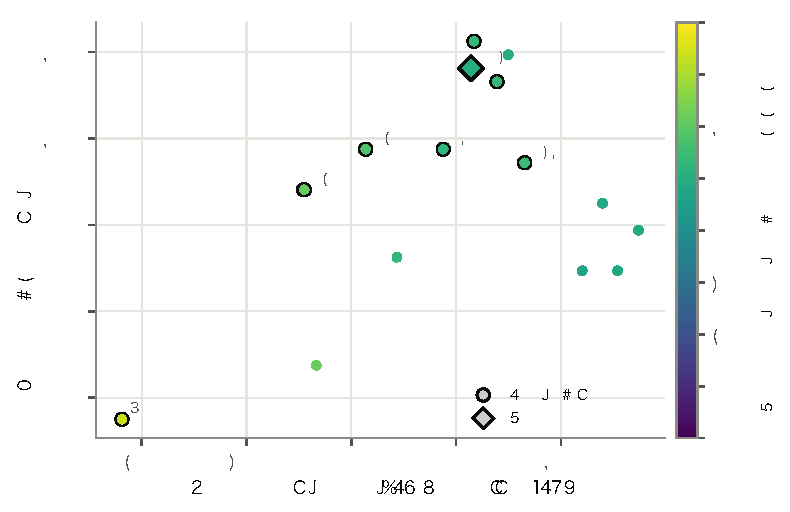
\includegraphics[width=0.66\textwidth]{figs/fig1_initial_actions.pdf}
\caption{Coverage and mean cumulative cost of each initial action (pathways under its recommended rule; 128 evaluation scenarios). Colour: remaining future options (mean over the period).}
\label{fig:init}
\end{figure}
\begin{itemize}
  \item 初期費用の小さい初期行動（施策なし・\#1・\#2）と、初期費用が大きく Coverage の高い初期行動（\#73・\#5）が、Coverage と費用のトレードオフの上に並ぶ（図\ref{fig:init}）。
    Coverage の上限は約 66\% で、施策の範囲と予算では Target を保てない将来が残る。
  \item 初期費用の小さい初期行動ほど、残る将来の選択肢が多い（施策なし 80\%、\#1 78\%、\#73 56\%）。
  \item 推奨ルールの多くは、被害の観測値・予測値と降雨の傾向を組み合わせて監視し、Target の 0.7〜0.9 倍で動く。降雨の傾向だけを監視するルール（\#81）は費用がかさむ。
  \item 基準の計算では \#73 が推奨された（評価シナリオで選んだ場合）。計画者の視点で探索シナリオから選ぶと、推奨は \#2 になる（\ref{sec:rq2}節）。
    両者の Coverage の差は小さく、推奨は選び方と探索の乱数に左右されうる。
\end{itemize}

\subsubsection*{推奨初期行動 \#73 と \#2 の経路の比較}
\begin{figure}[tbp]
\centering
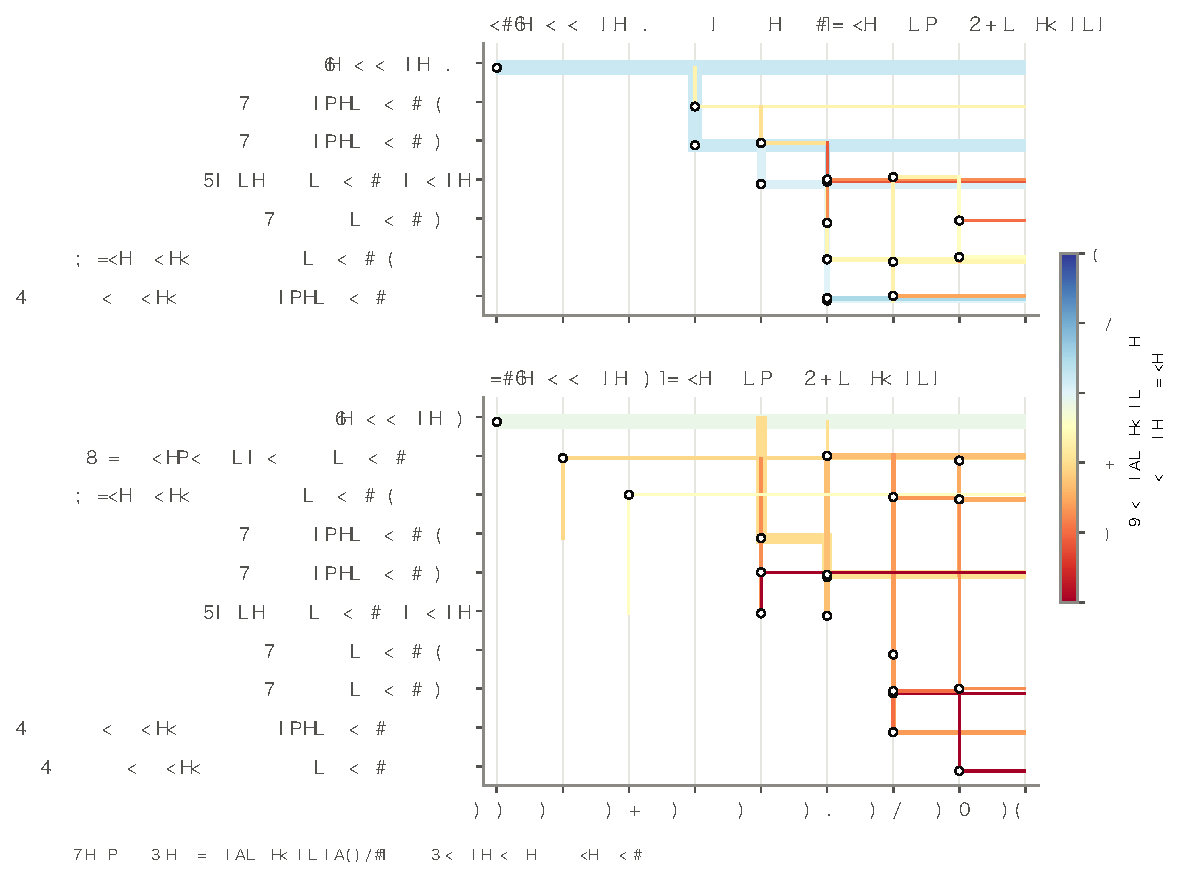
\includegraphics[width=0.95\textwidth]{figs/fig2_pathways_map.pdf}
\caption{Adaptive Pathways Maps of (a) the recommended initial action \#73 and (b) initial action \#2 (128 evaluation scenarios).
Rows: actions on individual measures; branches: differences in observations; colour: share of scenarios on the branch meeting the Target.
Rules: (a) monitors the observed and projected ratios and the rainfall trend, trigger 0.9 × Target, one action per decision;
(b) monitors the observed damage only, trigger 0.8 × Target, cost-weighted, up to two actions per decision.}
\label{fig:map}
\end{figure}
\begin{figure}[tbp]
\centering
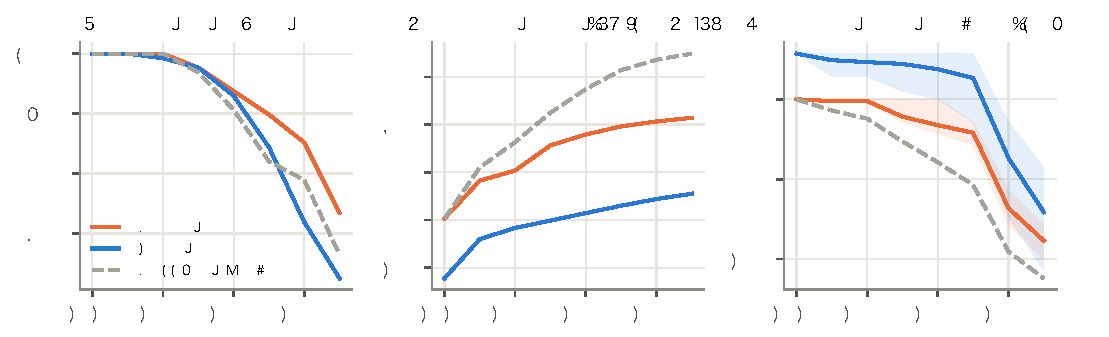
\includegraphics[width=0.98\textwidth]{figs/fig3_time_course.pdf}
\caption{Time course of \#73 and \#2 under their adaptive rules and, for reference, of the 11.9 pathway from \#73 (dashed):
share of scenarios meeting the Target up to each year, mean cumulative cost, and remaining future options (mean and 10--90\% range).}
\label{fig:time}
\end{figure}
\#73（初期費用 423 億円, Coverage 64\%, 平均費用 514 億円）と、初期費用の小さい Pareto 解 \#2（250 億円, 57\%, 355 億円）の経路を比べる
（図\ref{fig:map}・\ref{fig:time}）。\#73 は \#2 に中流の堤防 +2 m・上流の公共貯留・下流の各戸貯留を加えたもので、ルールも異なる。
\begin{itemize}
  \item \textbf{\#73（早めに備える型）}: 観測した比か現状のままの予測が Target の 0.9 倍を超えるか、観測した降雨の傾向が ×1.12 を超えたら、
    完成から 20 年後の予測効果を費用で割り引いた得点が最も高い行動を 1 つ実施する。主な分岐は 2050 年前後の下流堤防 +2 m（128 シナリオ中 108）で、
    多くは降雨の傾向で引き金が引かれ、被害が観測される前に動く（引き金の回数は降雨の傾向 218・観測 88・予測 83）。
    その後に上流の移転（64）、下流の排水機場（53）、上流の排水ポンプ（17）が続く。経路は行動の順序で 38 通りに分かれ、追加の行動は平均 3.0 回、
    追加の行動なしで Target を満たし続けたのは 7 シナリオ（5\%）である。2050 年までに失われる選択肢は 3\%（移転によって嵩上げができなくなる分）である。
  \item \textbf{\#2（様子を見る型）}: 被害の観測値だけを監視し、Target の 0.8 倍を超えたら費用を重視して 1 期に最大 2 行動を実施する。
    128 シナリオ中 36（28\%）は追加の行動なしで 2100 年まで Target を満たす。最初の主な分岐は 2060 年の下流堤防 +1 m（86）で、\#73 より 10 年遅く、規模も小さい。
    その後、下流堤防 +2 m（計 89）、上流の公共貯留（75）、上流の排水ポンプ（68）、上流の移転（49）、上流の堤防 +2 m（45）、下流・上流の排水機場（40・22）が、
    シナリオに応じてさまざまな順序で加わる。経路は 44 通りに分かれ、追加の行動は平均 4.0 回で、\#73 より多い。
  \item \textbf{時系列の違い}: 2060 年までは、Target を満たし続けたシナリオの割合はほぼ同じである（\#73 94\%、\#2 93\%）。
    2070 年以降に差が開き、2080 年に 85\% と 72\%、2090 年に 73\% と 62\% になる（図\ref{fig:time}）。
    \#2 は被害が観測されてから動くので、施工のリードタイム（堤防 6〜12 年）の間に Target を超える評価期が生じる。図\ref{fig:map}(b) の 2080 年以降の枝の多くが赤いのはこのためである。
    一方、2090 年までの平均累積費用は \#2 の方が約 160 億円少なく（約 355 億円と 514 億円）、残る将来の選択肢も 2070 年までは \#2 の方が多い（約 65〜72\% と 52〜60\%）。
  \item \textbf{解釈}: 二つは、早い段階の備え（初期投資と、降雨の傾向に基づく前倒しの嵩上げ）と、将来の柔軟性（安く始め、必要になったシナリオだけで施策を加える）の
    どちらを重視するかの違いである（RQ4）。\#2 の弱点は初期施策ではなく、遅く動くルールにある。全範囲（Low–High）で計画すると \#2 には予測値を監視して早めに（0.7 倍で）動くルールが選ばれ、
    Coverage は 66\%、平均費用は 440 億円になる（表\ref{tab:plan}）。初期投資を増やす代わりに、監視と引き金を前倒しすることで、\#73 と同程度の Coverage をより安く得られる。
  \item 参考として、同じ初期施策 \#73 から 11.9 方式の経路をとると、2090 年までの累積費用は約 650 億円で、Target を満たし続ける割合は 2080 年で 79\% である（図\ref{fig:time} の破線）。
\end{itemize}

\begin{figure}[tbp]
\centering
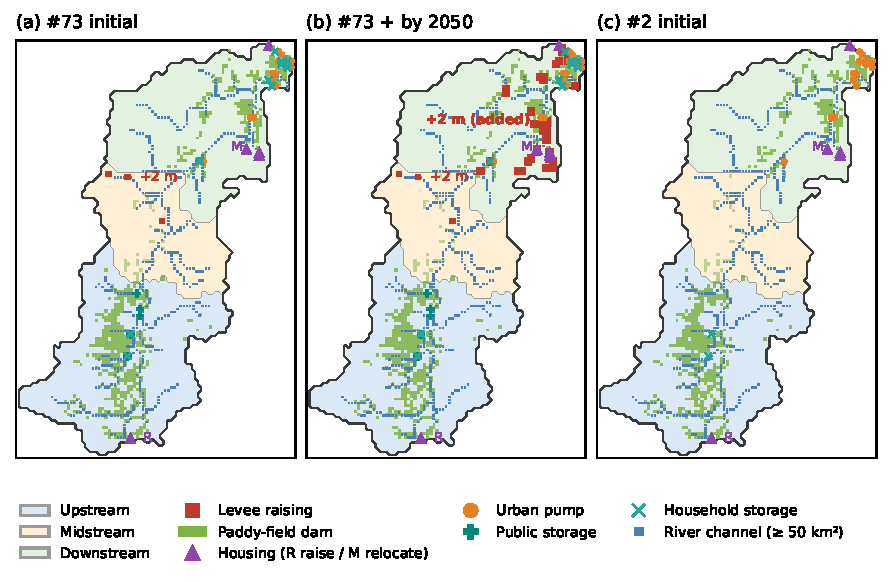
\includegraphics[width=0.98\textwidth]{figs/fig6_placement_v2.pdf}
\caption{Placement of the measures of (a) the recommended initial action \#73, (b) \#73 with the levee downstream +2 m added around 2050
(the first main branch, 108 of 128 scenarios; bold label), and (c) initial action \#2 (baseline run \texttt{abukuma\_dapp\_adaptive}, exploration v2).
Paddy-field dam: dark = 100\%, light = 50\% of the candidate cells. R = house raising, M = relocation.}
\label{fig:placement73}
\end{figure}
\begin{figure}[tbp]
\centering
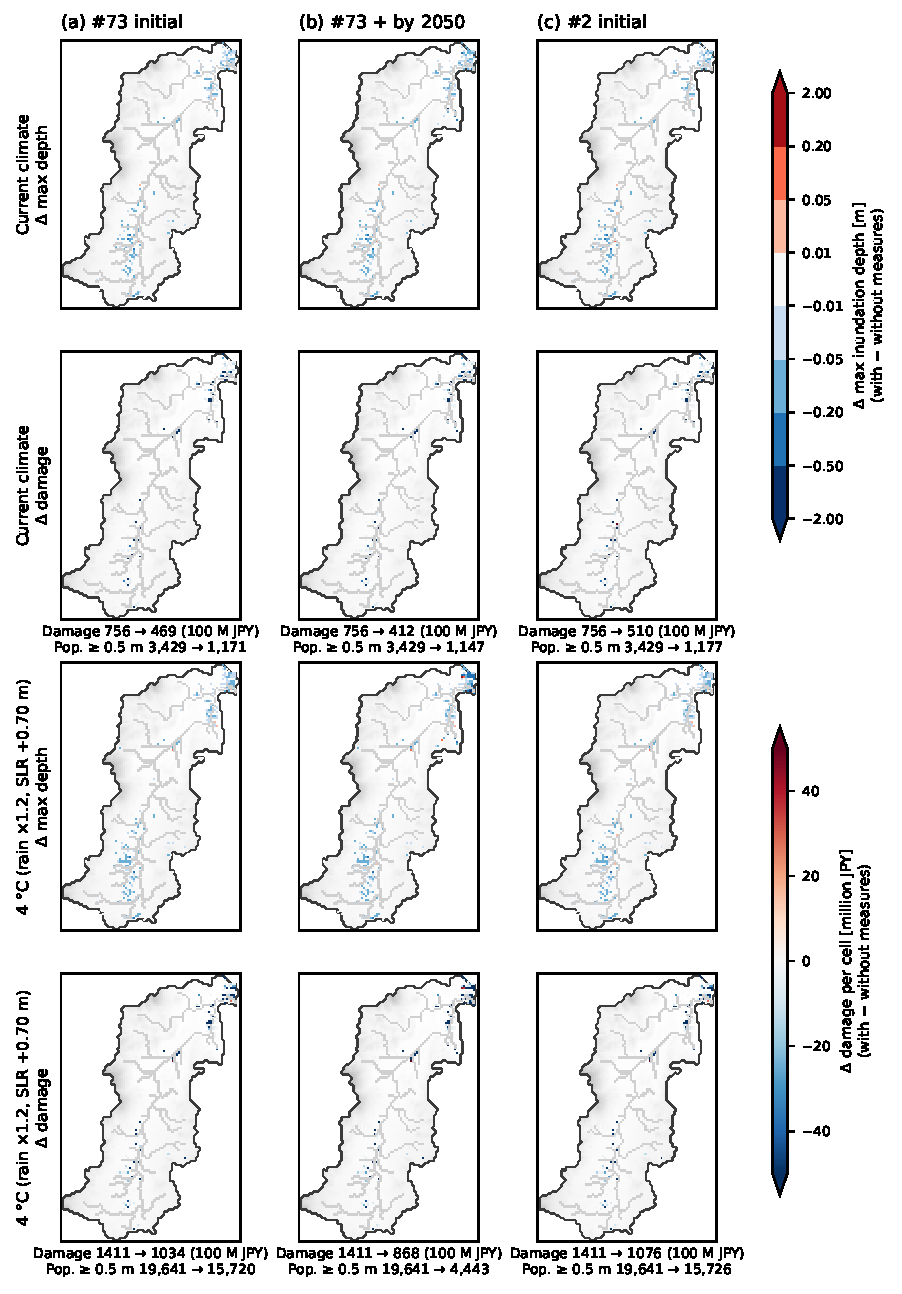
\includegraphics[width=0.9\textwidth]{figs/fig7_effect_maps_v2.pdf}
\caption{Simulated effect of the states of Fig.~\ref{fig:placement73} by the full RRI model (not the surrogate):
change in maximum inundation depth and in damage per 1-km cell (with − without measures) for the representative flood (Typhoon Hagibis, 2019)
under the current climate and 4\,°C (rainfall ×1.2, sea level +0.70 m), with the nominal effect coefficients
(levee 0.9, retention 0.85, paddy-field dam 0.6, afforestation 0.6, house raising 0.8).
Below each damage map: total damage and population in cells flooded ≥ 0.5 m, without → with measures.}
\label{fig:effect73}
\end{figure}
代理モデルを使うのは経路の探索だけなので、経路上の代表的な状態は RRI 本体で計算し直し、どこに何を置き、どこで浸水と被害が減るかを地図で確かめられる。施策の配置と、その効果を RRI 本体で計算し直した結果を図\ref{fig:placement73}・\ref{fig:effect73}に示す（代表洪水 1 つ、効果係数は標準値）。
\begin{itemize}
  \item \textbf{配置}: 両者とも上流・下流の田んぼダム、上流の住宅の嵩上げ、下流の移転、下流の排水ポンプを含む。\#73 はこれに中流の堤防 +2 m（短い区間）、
    上流の公共貯留（市街地 5 セル）、下流の各戸貯留を加える。2050 年前後の追加は下流の本川沿いの堤防 +2 m である。
  \item \textbf{現在気候}: 施策なしの被害額 756 億円に対し、\#73 で 469 億円、\#2 で 510 億円、\#73 に下流堤防を加えた状態で 412 億円である。
    浸水深 0.5 m 以上の人口は 3 状態とも約 1,150〜1,180 人（施策なし 3,429 人）でほとんど差がない。\#73 が \#2 より多く減らすのは、上流の被害（$-117$ 億円と $-97$ 億円）と下流の被害（$-168$ 億円と $-147$ 億円）の両方である。
  \item \textbf{4\,℃}: 施策なしの 1,411 億円・19,641 人に対し、\#73 で 1,034 億円・15,720 人、\#2 で 1,076 億円・15,726 人と、初期行動の差は小さい。
    下流堤防 +2 m を加えると 868 億円・4,443 人になり、下流の被害の減少は 217 億円から 411 億円に増える（図\ref{fig:effect73} 下 2 段の (b)）。
    初期行動の違いより、下流堤防をいつ加えるかの方が、強い降雨での結果を大きく左右する。\#73 のルールが降雨の傾向を見て 2050 年前後に下流堤防を前倒しし、\#2 のルールが被害の観測を待って 2060 年に +1 m から始めることが、
    2070 年以降の Target を満たす割合の差（図\ref{fig:time}）につながる。
  \item 下流堤防を加えた 4\,℃ の状態では、上流の被害の減少が \#73 の初期状態より約 30 億円小さい（$-131$ 億円と $-160$ 億円）。浸水深が 5 cm 以上増えたセルは 4 セル（最大 0.23 m）だけであり、
    この差がどこから来るか（河道の水位の変化か、計算の揺らぎか）は確認していない。
\end{itemize}

\subsubsection*{施策の配置と、RRI で計算した効果の地図（v4）}
\begin{figure}[tbp]
\centering
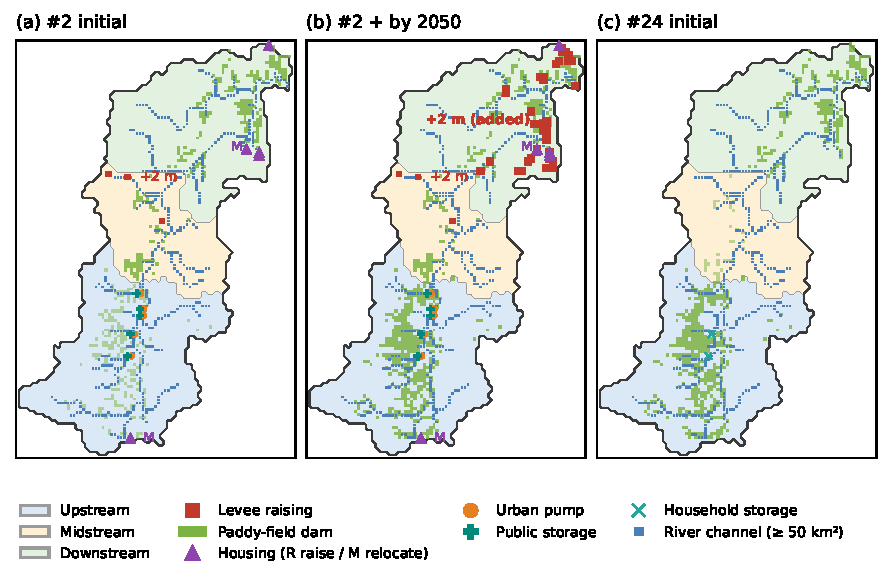
\includegraphics[width=0.98\textwidth]{figs/fig6_placement.pdf}
\caption{Placement of the measures (exploration v4, run \texttt{abukuma\_dapp\_adaptive\_v4}).
(a) Recommended initial action \#2 of v4; (b) \#2 with the most frequent additions by 2050 on its pathway
(paddy-field dam upstream 50 → 100\%, 113 of 128 scenarios, 2030; levee downstream +2 m, 82 scenarios, ~2050; bold labels);
(c) low-cost Pareto initial action \#24. Paddy-field dam and afforestation: dark = 100\%, light = 50\% of the candidate cells.
R = house raising, M = relocation. Numbering of the initial actions differs from v2 (Table~\ref{tab:initacts}).}
\label{fig:placement}
\end{figure}
\begin{figure}[tbp]
\centering
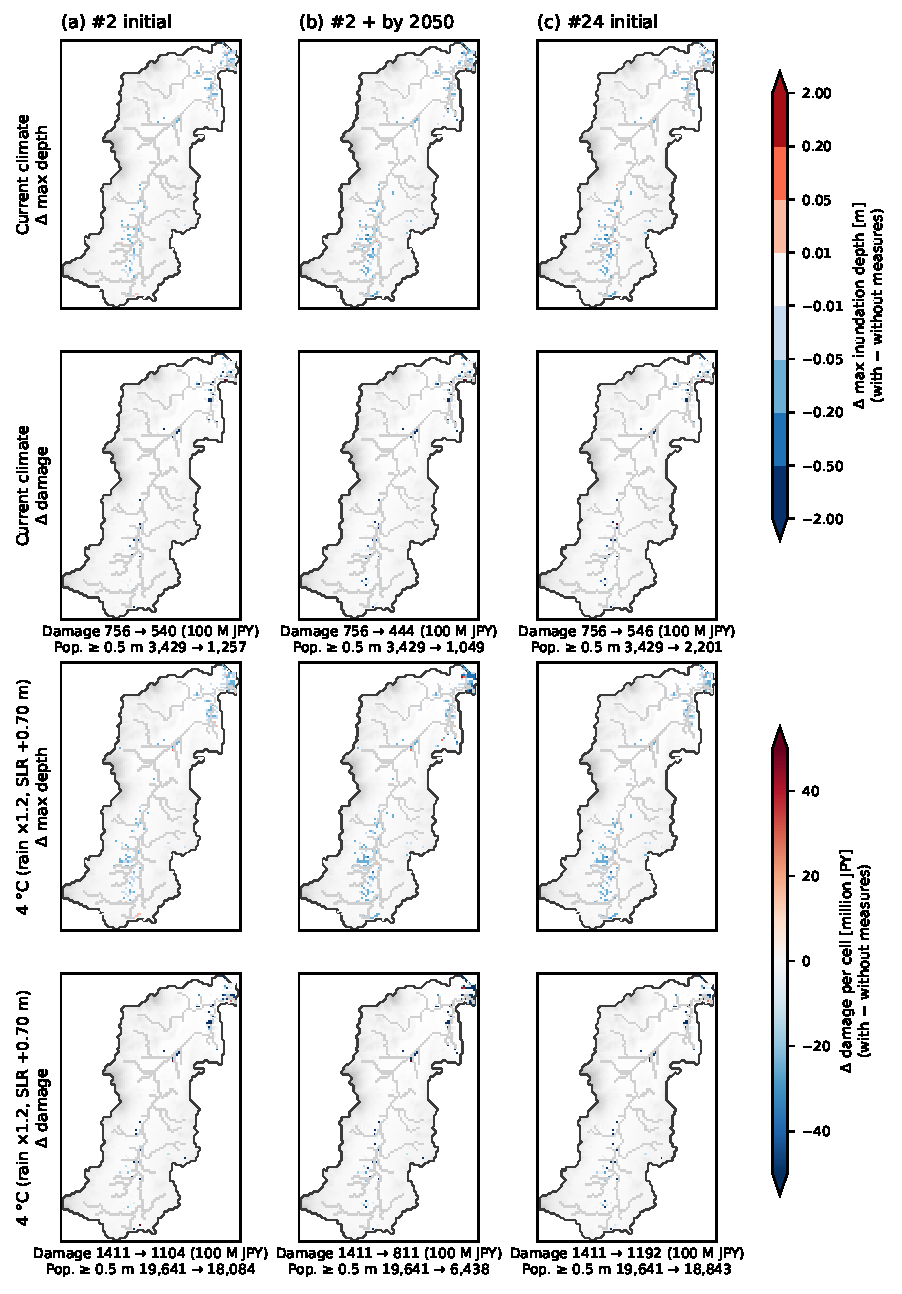
\includegraphics[width=0.9\textwidth]{figs/fig7_effect_maps.pdf}
\caption{Simulated effect of the states of Fig.~\ref{fig:placement} by the full RRI model (not the surrogate):
change in maximum inundation depth and in damage per 1-km cell (with − without measures) for the representative flood (Typhoon Hagibis, 2019)
under the current climate and 4\,°C (rainfall ×1.2, sea level +0.70 m), with the nominal effect coefficients
(levee 0.9, retention 0.85, paddy-field dam 0.6, afforestation 0.6, house raising 0.8).
Below each damage map: total damage and population in cells flooded ≥ 0.5 m, without → with measures.}
\label{fig:effectmap}
\end{figure}
同じ地図を、遊水地を計画中の上流遊水地群に置き換えた v4 の結果でも作った（初期行動の番号は v2 と異なる）。
v4 の推奨初期行動 \#2（初期費用 257 億円, Coverage 68\%, 平均費用 358 億円）は、中流の堤防 +2 m、上流・中流・下流の田んぼダム、上流・下流の住宅の移転、
上流の排水ポンプと公共貯留からなる。その経路では、2030 年に上流の田んぼダムを 100\% に広げ（128 シナリオ中 113）、
2050 年前後に下流の堤防を +2 m 上げる（82）のが主な流れである。比較には、安く始めて必要になってから加える Pareto 解 \#24
（田んぼダムと上流の各戸貯留, 初期費用 38 億円, Coverage 63\%, 平均費用 240 億円）を用いた（図\ref{fig:placement}）。
上流が流域の南側、下流（河口側）が北側である。
\begin{itemize}
  \item \textbf{現在気候}: 施策なしの被害額 756 億円（上流 277・下流 474）に対し、\#2 の初期状態で 540 億円、2050 年までの追加後で 444 億円、\#24 で 546 億円である。
    \#2 と \#24 の被害額の差は小さいが、浸水深 0.5 m 以上の人口は \#2 で 1,257 人、\#24 で 2,201 人（施策なし 3,429 人）であり、
    \#2 の住宅の移転が人の被害を減らしている。浸水深が下がるのは、主に上流の水田地帯（田んぼダム）と下流の低地である（図\ref{fig:effectmap} 上 2 段）。
  \item \textbf{4\,℃}: 施策なしの被害額は 1,411 億円（下流 977）、浸水深 0.5 m 以上の人口は 19,641 人に増える。
    \#2 の初期状態（1,104 億円, 18,084 人）と \#24（1,192 億円, 18,843 人）では人口がほとんど減らないのに対し、
    下流堤防 +2 m を加えた状態では 811 億円、6,438 人になる。減った被害額 600 億円のうち 380 億円が下流で、河口側の市街地の浸水が大きく減る（図\ref{fig:effectmap} 下 2 段の (b)）。
    現在気候では下流堤防の追加による下流の被害の減少は約 40 億円にとどまるので、下流堤防は降雨が増えるほど効果が大きくなる施策であり、多くのシナリオで降雨の傾向や被害の観測を見てから 2050 年前後に選ばれることと整合する。
  \item \textbf{浸水が増える場所}: 堤防の嵩上げで水が下流や対岸に移ることがありうる。今回の状態では浸水深が 5 cm 以上増えたセルは各ケース 0〜4 セル（最大 0.23 m, 4\,℃ の (b) の下流）で、
    被害額の増加は合計 0.7〜3.3 億円と、減少分に比べて小さい。
  \item \textbf{注意}: 地図は 1 つの代表洪水・2 つの気候・効果係数の標準値での結果であり、128 シナリオでの Coverage を表すものではない。
    また 1 km 格子のため、堤防の区間や移転先は格子単位の近似である。
\end{itemize}

\subsection{RQ2: 考慮する気候の幅と望ましい経路}
\label{sec:rq2}
\label{sec:plan}
\begin{table}[H]
\centering\footnotesize\setlength{\tabcolsep}{3pt}
\caption{Recommended DAPP for each planning climate range (standard: 24 search scenarios, default Target; Coverage and cost over the 128 evaluation scenarios; numbers of scenarios in parentheses; Lock-in in 2050)}
\label{tab:plan}
\begin{tabularx}{\textwidth}{@{}>{\raggedright\arraybackslash}p{25mm} l L r r >{\raggedright\arraybackslash}p{22mm} r r r r@{}}
\toprule
Range (rainfall / sea level) & Rec. & Rule & All & Within & Outside (more severe / milder) & Expected\textsuperscript{a} & Cost & Remaining & Lock-in \\
\midrule
Low (1.0--1.1 / 0.20--0.38 m) & \#2 & Observed; $\rho$ 0.8 & 53\% & 100\% (12) & 48\% (116) / -- & 100\% & 345 & 62\% & 2.9\% \\
Medium (1.1--1.2 / 0.38--0.54) & \#2 & Observed; $\rho$ 0.7 & 66\% & 77\% (13) & 44\% (71) / 98\% (44) & 83\% & 432 & 58\% & 2.9\% \\
High (1.2--1.3 / 0.54--0.70) & \#2 & Observed, projected; $\rho$ 0.7 & 70\% & 33\% (12) & -- / 74\% (116) & 42\% & 523 & 54\% & 2.9\% \\
Low--High (full range) & \#2 & Projected; $\rho$ 0.7 & 66\% & 66\% & -- & 71\% & 440 & 57\% & 2.9\% \\
\bottomrule
\end{tabularx}
\par\footnotesize \textsuperscript{a} Coverage expected at planning (over the search scenarios inside the planning range).
\end{table}
\begin{itemize}
  \item 推奨される初期行動はどの範囲でも \#2（250 億円）である。変わるのはその後のルールで、Low では被害の観測値だけを監視して遅めに（Target の 0.8 倍で）動き、
    High では予測値も監視して早めに（0.7 倍で）動く。
  \item 厳しい気候を考えるほど、平均費用は増え（Low 345 → High 523 億円）、残る将来の選択肢は減る（62\% → 54\%）。追加の施策を早く使うためである。
  \item 評価シナリオの上で最良だった初期行動（事後に最良）は Low で \#90、Medium で \#64 で、計画者の視点で選んだ \#2 との Coverage の差は 3〜4 pt である。
\end{itemize}

\subsection{RQ3: 共通の評価シナリオでの性能}
\begin{figure}[H]
\centering
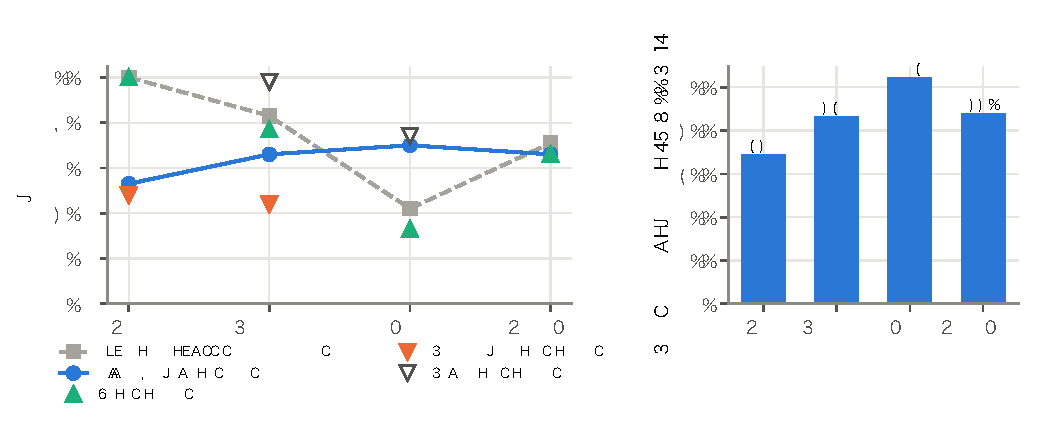
\includegraphics[width=0.9\textwidth]{figs/fig4_planning_range.pdf}
\caption{Coverage of the recommended DAPP by planning climate range (expected at planning, all, within and outside the range) and mean cost (128 evaluation scenarios).}
\label{fig:plan}
\end{figure}
\begin{itemize}
  \item 全体の Coverage は Low 53\%・Medium 66\%・High 70\%・Low–High 66\% である（表\ref{tab:plan}、図\ref{fig:plan}）。
  \item \textbf{計画時の見込みとの差}: Low で設計した経路は、計画時には 100\% と見込まれるが、全体では 53\%、範囲より厳しい将来では 48\% にとどまる（過信）。
    High では逆に、見込み 42\% に対して全体では 70\% になる（悲観）。Low–High では見込み 71\% と評価 66\% の差が最も小さい。
  \item High で設計しても、範囲内（4℃ 以上）の将来での Coverage は 33\% である。この施策の範囲と予算では、厳しい気候の下で Target を保てない将来が残る。
  \item 平均費用あたりの Coverage は、Medium と Low–High（66\%、432〜440 億円）が High（70\%、523 億円）より効率的である。
\end{itemize}

\subsection{RQ4: 目標の水準と、早い段階の備え・将来の柔軟性}
\begin{table}[H]
\centering\footnotesize\setlength{\tabcolsep}{4pt}
\caption{Recommended initial action by planning climate range × Target (fast setting: 12 search scenarios; flooded-population Target 1.5 ×). Initial cost [100 M JPY] · Coverage (128 evaluation scenarios) · mean cost [100 M JPY] · remaining future options (mean)}
\label{tab:target}
\begin{tabular}{@{}lccc@{}}
\toprule
Planning range & Damage Target 1.0 × (strict) & 1.2 × (default) & 1.4 × (lenient) \\
\midrule
Low & \#2: 250 · 38\% · 335 · 63\% & \#2: 250 · 46\% · 295 · 64\% & \#73: 423 · 60\% · 448 · 54\% \\
Medium & \#2: 250 · 41\% · 331 · 63\% & \#1: 197 · 52\% · 343 · 70\% & \#73: 423 · 75\% · 621 · 47\% \\
High & \#1: 197 · 34\% · 307 · 73\% & \#81: 377 · 70\% · 764 · 41\% & \#26: 125 · 70\% · 562 · 47\% \\
Low--High & \#2: 250 · 48\% · 480 · 56\% & \#25: 101 · 60\% · 436 · 56\% & \#73: 423 · 73\% · 532 · 50\% \\
\bottomrule
\end{tabular}
\end{table}
\begin{figure}[H]
\centering
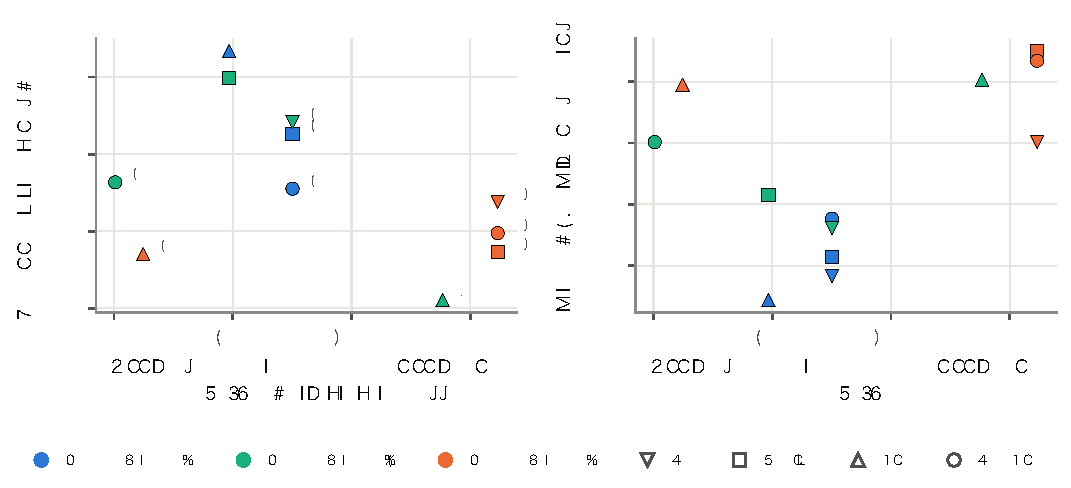
\includegraphics[width=0.98\textwidth]{figs/fig5_target_preparedness.pdf}
\caption{Initial cost of the recommended initial action (early preparedness) versus remaining future options (left) and Coverage (right). Colour: Target; marker: planning climate range.}
\label{fig:target}
\end{figure}
\begin{itemize}
  \item 目標の水準は、考慮する気候の幅よりも推奨を大きく変える（表\ref{tab:target}、図\ref{fig:target}）。
  \item \textbf{緩い目標（1.4 倍）}: 4 範囲のうち 3 範囲で、初期費用の大きい \#73（423 億円）が推奨される。Coverage は 60〜75\% と高いが、残る将来の選択肢は 47〜54\% に減る。
    早く備えれば守れる将来が多いので、初期に投資する価値が高い。
  \item \textbf{厳しい目標（1.0 倍）}: どの初期行動でも Target を保てる将来が少ない（Coverage 34〜48\%）。そのため推奨は初期費用の小さい \#1・\#2 になり、残る将来の選択肢は 56〜73\% と多い。
    守れない将来の多い目標に対しては、早く投資するより、選択肢を残して観測を待つ経路が選ばれる。
    補足として、被害額・浸水人口とも 1.1 倍とし High の範囲で計画すると、推奨は「施策なし」になる（Coverage 24\%、標準計算）。
  \item この傾向は、推奨の選び方（最高の Coverage から 3 pt 以内で最も安い）にも左右される。厳しい目標では初期行動の間の Coverage の差が小さく、安い初期行動が選ばれやすい。
  \item 例外として、High と緩い目標の組合せでは森林化を含む \#26（125 億円）が推奨され、Lock-in が 10.8\% と大きい（他は 2.9\% 前後）。
  \item 簡易計算では、推奨初期行動が条件ごとに入れ替わりやすい（Target 既定の行で \#2・\#1・\#81・\#25）。標準計算では Target 既定のとき 4 範囲とも \#2 であった。結論には標準計算で確かめる必要がある。
\end{itemize}

\subsection{補足: 監視情報の質}
\begin{table}[H]
\centering\small
\caption{Sensitivity to information quality (recommended rules of the baseline run fixed and re-evaluated; 128 evaluation scenarios; mean over all initial actions)}
\label{tab:sens}
\begin{tabular}{@{}lrr@{}}
\toprule
Condition & Mean Coverage & Mean cost [100 M JPY] \\
\midrule
Baseline & 57\% & 492 \\
Observation errors × 0 (perfect observation) & 58\% & 485 \\
Observation errors × 3 / × 6 & 57\% / 57\% & 529 / 557 \\
Projection error $\sigma$ 0.5 / 1.0 & 57\% / 56\% & 500 / 507 \\
Observations for trend estimation 2 / 5 & 56\% / 56\% & \\
\midrule
(For comparison) damage Target 1.0 / 1.4 × & 43\% / 62\% & \\
(For comparison) flooded-population Target 1.2 × & 50\% & \\
\bottomrule
\end{tabular}
\end{table}
\begin{itemize}
  \item 監視情報の質を大きく変えても、平均 Coverage の変化は 1〜2 pt である（表\ref{tab:sens}）。観測誤差が大きいと、誤って早く動く分だけ費用が増える（485 → 557 億円）。
  \item ルールを探索し直しても同じ傾向である（Target 1.0 倍・浸水人口 1.0 倍、簡易計算: 観測誤差 × 1 で 45\%、× 2 で 45\%）。
  \item この流域・この施策の範囲では、Coverage を決めるのは情報の質より目標の水準と施策の範囲である。
\end{itemize}

\subsection{補足: 比較の基準（11.9 方式）との関係}
同じ初期行動・同じ評価シナリオで 11.9 方式の経路をとると、平均 Coverage は 49\%（適応ルールは 57\%）、平均費用は 528 億円（同 492 億円）である。
差の大きさは初期行動によって異なり（表\ref{tab:init}）、\#2 では両者はほぼ同じである。11.9 方式の結果は、適応ルールの水準を読むための参照点として示すにとどめる。

%=====================================================================
\section{議論と限界}
\label{sec:discussion}
\begin{itemize}
  \item \textbf{計画時の想定の選び方}: 狭い範囲で設計すると、計画時の見込みが実際の性能から大きく外れる（Low で 47 pt の過大、High で 28 pt の過小）。
    推奨初期行動は範囲にあまり左右されないので、計画時の想定は主に「どの情報を監視し、どの水準で動くか」に反映される。
    全範囲で設計すると、見込みと評価の差が最も小さく、費用も中程度である。
  \item \textbf{目標の水準}: 目標を厳しくすると、守れない将来が増えて初期投資の価値が下がり、選択肢を残す経路が選ばれる。
    この結果は推奨の選び方に依存するので、目標の水準と許容する Coverage の差（3 pt）をあわせて示す必要がある。
  \item \textbf{将来の柔軟性の指標}: Remaining Future Options は施策の水準の数で数えた余地であり、施策ごとの効果や費用の大きさを反映しない。Lock-in も 2050 年の一時点の値である。補助的な指標として扱う。
  \item \textbf{初期行動の網羅性}: 経路全体で評価した初期行動は 16 に限られる（初期費用 500 億円以下の非劣解 649 から、静的な指標で選んだもの）。
    後から施策を足しやすい初期行動が漏れている可能性がある。\todo{候補を 64 に広げる、または既定ルールで粗く評価して上位だけ探索する}
  \item \textbf{ルールの探索}: 約 23 万通りのうち、初期行動ごとに約 110 を評価しただけである。推奨ルールは乱数の種で揺れうる（簡易計算では推奨初期行動が入れ替わる）。\todo{種を変えた反復}
  \item \textbf{ルールの形}: 監視指標 3 つ・1 つの得点式・格子は仮定である。より柔軟な形（直接方策探索 EMODPS\cite{giuliani2016,quinn2017} など）との比較が必要である。
  \item \textbf{物理モデルと代理モデル}: 代表洪水は 1 つで、代理モデルの誤差は ±25 億円程度、学習範囲の外へは外挿しない。小さい施策の効果は誤差に埋もれる。
    施策を 1 つだけ入れた状態で RRI と比べると（v3・v4, 22 ケース）、代理モデルは単独効果の順位を再現する（相関 0.94〜0.97）が、大きさを過小評価する
    （RRI に対する比の中央値 0.48〜0.53; 例: 中流堤防 +2 m は RRI で $-27$ 億円、代理モデルで $\pm0$）。
    単独効果を RRI で直接与え、組合せの効果だけを学習する構造に改める必要がある。
  \item \textbf{パラメータ}: 土地利用クラスは事前値で、施策のパラメータ（田んぼダムの貯留深と放流強度、森林化の土層厚と粗度、排水強度、貯留深）と費用の単価の多くは仮定である（\ref{sec:formulation}節）。
    森林化の効果は効果係数に対して単調でない（係数 0.5 の方が効果の大きい地域がある）。畑の浸透量の上限 $F_{\max}=0.3$ m と新規森林の土壌貯留 $0.4D$ の大小が係数によって入れ替わるためと考えられる。
  \item \textbf{遊水地}: 基準の計算（v2）の遊水地は自動選定した下流の 3 か所である。計画中の上流遊水地群に置き換えた v3・v4 では、遊水地群は初期行動に選ばれず、経路の途中で選ばれることも少ない。
    単独効果（RRI で $-28$ 億円）に対して初期費用（497 億円）が大きいためと考えられる。
  \item \textbf{社会過程}: 合意の失敗・参加率・主体間の調整は扱わない（11.10 の Multi-Actor DAPP で扱う）。
  \item \textbf{範囲内の標本}: Low・Medium・High の範囲内にある評価シナリオは 12〜13 と少なく、範囲内の Coverage の精度は低い。
\end{itemize}

%=====================================================================
\section{結論}
\label{sec:conclusion}
\begin{enumerate}
  \item \textbf{RQ1}: 初期行動と状態依存の適応ルールを同時に探索すると、初期費用の小さい初期行動（0〜250 億円）と大きい初期行動（約 425 億円）が Coverage と費用のトレードオフの上に並ぶ。
    望ましいルールは、被害の観測値・予測値と降雨の傾向を組み合わせて監視し、Target に達する前（0.7〜0.9 倍）に動く。
  \item \textbf{RQ2}: 計画時に考慮する気候の幅は、推奨する初期行動よりも、その後のルール（何を監視し、いつ動くか）を変える。厳しい気候を考えるほど、早く動き、費用が増え、将来の選択肢を早く使う。
  \item \textbf{RQ3}: 狭い気候の幅で設計した経路は、共通の評価シナリオでの性能が計画時の見込みから大きく外れる。全範囲で設計した経路は、見込みと実際の差が最も小さい。
  \item \textbf{RQ4}: 目標の水準は気候の幅よりも推奨を大きく変える。緩い目標では早い段階の備え（初期投資）が選ばれ、厳しい目標では選択肢を残して観測を待つ経路が選ばれる。
  \item 監視情報の質の影響は小さい。11.9 方式（あらかじめ与えた経路網）は参照点として示し、優劣の比較は論文の主張にしない。
\end{enumerate}

%=====================================================================
\section{今後の計算と論文化の作業}
\label{sec:next}
\begin{enumerate}
  \item 表と図を v4（上流遊水地群・施策の少ない学習点を追加した探索 \texttt{abukuma\_explore\_v4}）の結果で置き換える。v4 の基準の計算では、推奨初期行動の Coverage は 68\%、平均費用は 358 億円である。
  \item 代理モデルの単独効果の過小評価を改善し（単独効果を RRI で直接与える構造）、主要な結果を再計算する。
  \item planning range × Target の格子を標準計算（探索 24 シナリオ）で行い、乱数の種を変えて推奨の安定性を示す。
  \item 初期行動の候補を広げる。代表的な分岐状態を RRI で再評価（\texttt{--verify}）し、代理モデルの誤差を示す。
  \item 投稿先の候補: \todo{Environmental Modelling \& Software／Water Resources Research／Climate Risk Management／土木学会論文集（水工学）}
\end{enumerate}

\subsection*{再現手順}
\begin{verbatim}
python scripts/run_explore.py ...            # 探索（docs/12）: abukuma_explore_v2
python data/processed/explore/run_v4.py      # v4（上流遊水地群・施策の少ない学習点）
python scripts/run_roadmap.py --prepare      # 費用表・代理モデルのキャッシュ
python scripts/run_dapp.py --robust          # 11.9（初期行動の候補・参照の経路網）
python scripts/run_dapp.py --adaptive        # 11.11（ルールの探索と評価）
# planning range・Target・情報の質: GUI /dapp の Adaptive の実行から Recalculate
python docs/paper/dapp/measure_effects.py    # 表 5 の単独効果
python docs/paper/dapp/make_figs.py          # 図
\end{verbatim}

%=====================================================================
\begin{thebibliography}{99}\small
\bibitem{sayama2012} Sayama, T., Ozawa, G., Kawakami, T., Nabesaka, S., Fukami, K. (2012): Rainfall–runoff–inundation analysis of the 2010 Pakistan flood in the Kabul River basin, \textit{Hydrological Sciences Journal}, 57(2), 298--312.
\bibitem{bates2010} Bates, P.D., Horritt, M.S., Fewtrell, T.J. (2010): A simple inertial formulation of the shallow water equations for efficient two-dimensional flood inundation modelling, \textit{Journal of Hydrology}, 387(1--2), 33--45.
\bibitem{greenampt1911} Green, W.H., Ampt, G.A. (1911): Studies on soil physics, Part I: The flow of air and water through soils, \textit{Journal of Agricultural Science}, 4(1), 1--24.
\bibitem{honma1940} 本間仁 (1940): 低溢流堰堤の流量係数, 土木学会誌, 26(6), 635--645; 26(9), 849--862.
\bibitem{renno2008} Rennó, C.D., Nobre, A.D., Cuartas, L.A., et al. (2008): HAND, a new terrain descriptor using SRTM-DEM: Mapping terra-firme rainforest environments in Amazonia, \textit{Remote Sensing of Environment}, 112(9), 3469--3481.
\bibitem{nobre2011} Nobre, A.D., Cuartas, L.A., Hodnett, M., et al. (2011): Height Above the Nearest Drainage -- a hydrologically relevant new terrain model, \textit{Journal of Hydrology}, 404(1--2), 13--29.
\bibitem{mlit_manual} 国土交通省 水管理・国土保全局 (2025): 治水経済調査マニュアル（案）（令和 7 年 6 月改正）.
\bibitem{mlit_usuichi} 国土交通省 東北地方整備局 福島河川国道事務所: 阿武隈川上流遊水地群の概要, \url{https://www.thr.mlit.go.jp/fukushima/usuichi_faq/1-1-1_sisetugaiyou.pdf}（2026 年 11 月閲覧）.
\bibitem{mlit_teigen} 気候変動を踏まえた治水計画に係る技術検討会 (2021): 気候変動を踏まえた治水計画のあり方 提言（改訂版）, 国土交通省.
\bibitem{mlit_ryuiki} 社会資本整備審議会 (2020): 気候変動を踏まえた水災害対策のあり方について ～あらゆる関係者が流域全体で行う持続可能な「流域治水」への転換～（答申）.
\bibitem{jma2020} 文部科学省・気象庁 (2020): 日本の気候変動 2020 －大気と陸・海洋に関する観測・予測評価報告書－.
\bibitem{maff_tanbo} 農林水産省 農村振興局 (2022): 「田んぼダム」の手引き.
\bibitem{scj2001} 日本学術会議 (2001): 地球環境・人間生活にかかわる農業及び森林の多面的な機能の評価について（答申）.
\bibitem{kuraji2004} 蔵治光一郎・保屋野初子 編 (2004): 緑のダム ―森林・河川・水循環・防災―, 築地書館.
\bibitem{ksj} 国土交通省: 国土数値情報（土地利用細分メッシュ L03-b、行政区域 N03、国有林野 A45）.
\bibitem{haasnoot2013} Haasnoot, M., Kwakkel, J.H., Walker, W.E., ter Maat, J. (2013): Dynamic adaptive policy pathways: A method for crafting robust decisions for a deeply uncertain world, \textit{Global Environmental Change}, 23(2), 485--498.
\bibitem{kwadijk2010} Kwadijk, J.C.J., Haasnoot, M., Mulder, J.P.M., et al. (2010): Using adaptation tipping points to prepare for climate change and sea level rise: a case study in the Netherlands, \textit{WIREs Climate Change}, 1(5), 729--740.
\bibitem{lempert2003} Lempert, R.J., Popper, S.W., Bankes, S.C. (2003): \textit{Shaping the Next One Hundred Years: New Methods for Quantitative, Long-Term Policy Analysis}, RAND, MR-1626.
\bibitem{kwakkel2016} Kwakkel, J.H., Haasnoot, M., Walker, W.E. (2016): Comparing Robust Decision-Making and Dynamic Adaptive Policy Pathways for model-based decision support under deep uncertainty, \textit{Environmental Modelling \& Software}, 86, 168--183.
\bibitem{giuliani2016} Giuliani, M., Castelletti, A., Pianosi, F., Mason, E., Reed, P.M. (2016): Curses, tradeoffs, and scalable management: Advancing evolutionary multiobjective direct policy search to improve water reservoir operations, \textit{Journal of Water Resources Planning and Management}, 142(2), 04015050.
\bibitem{quinn2017} Quinn, J.D., Reed, P.M., Keller, K. (2017): Direct policy search for robust multi-objective management of deeply uncertain socio-ecological tipping points, \textit{Environmental Modelling \& Software}, 92, 125--141.
\bibitem{haasnoot2018} Haasnoot, M., van 't Klooster, S., van Alphen, J. (2018): Designing a monitoring system to detect signals to adapt to uncertain climate change, \textit{Global Environmental Change}, 52, 273--285.
\bibitem{hermans2017} Hermans, L.M., Haasnoot, M., ter Maat, J., Kwakkel, J.H. (2017): Designing monitoring arrangements for collaborative learning about adaptation pathways, \textit{Environmental Science \& Policy}, 69, 29--38.
\bibitem{deb2002} Deb, K., Pratap, A., Agarwal, S., Meyarivan, T. (2002): A fast and elitist multiobjective genetic algorithm: NSGA-II, \textit{IEEE Transactions on Evolutionary Computation}, 6(2), 182--197.
\bibitem{mckay1979} McKay, M.D., Beckman, R.J., Conover, W.J. (1979): A comparison of three methods for selecting values of input variables in the analysis of output from a computer code, \textit{Technometrics}, 21(2), 239--245.
\bibitem{rasmussen2006} Rasmussen, C.E., Williams, C.K.I. (2006): \textit{Gaussian Processes for Machine Learning}, MIT Press.
\end{thebibliography}

\end{document}
